% LaTeX source for book ``模形式初步'' in Chinese
% Copyright 2020  李文威 (Wen-Wei Li).
% Permission is granted to copy, distribute and/or modify this
% document under the terms of the Creative Commons
% Attribution 4.0 International (CC BY 4.0)
% http://creativecommons.org/licenses/by/4.0/

\chapter{基本定义}
对上半平面 $\mathcal{H}$ 赋予 Riemann 度量 $\frac{\dd x^2 + \dd y^2}{y^2}$, 其曲率为常数 $-1$, 这是双曲几何常见的模型. 具有整数权 $k$ 和级 $\SL(2,\Z)$ 的模形式是定义在 $\mathcal{H}$ 上的一类全纯函数, 按定义, 这样一个函数 $f$ 必须
\begin{enumerate}[(a)]
	\item 满足 $(c\tau + d)^{-k} f\left( \dfrac{a\tau+b}{c\tau+d} \right) = f(\tau)$, 其中 $\twomatrix{a}{b}{c}{d}$ 取遍 $\SL(2,\Z)$, 
	\item 具有 Fourier 展开 $f(\tau) = \sum_{n \geq 0} a_n(f) q^n$, 其中 $q := e^{2\pi i\tau}$; Fourier 系数 $a_n(f)$ 往往蕴藏微妙的算术信息.
\end{enumerate}
这里的作用 $\left( \twomatrix{a}{b}{c}{d}, \; \tau \right) \mapsto \frac{a\tau+b}{c\tau+d}$ 是复变函数论中熟知的线性分式变换. 实用中需要比 $\SL(2,\Z)$-作用更宽松的对称性, 或谓更深的``级'', 并研究模形式在所谓``尖点''附近的性状. 上半平面在离散子群作用下的基本区域扮演举足轻重的角色, 相关定义见 \S\ref{sec:fundamental-domain}. 复变函数论, 群论与双曲几何在此熔于一炉.

千头万绪, 本章且先从上半平面的几何性质入手, 然后确定 $\SL(2,\Z)$ 的基本区域, 定义同余子群及其尖点. 掌握这些概念便能定义以任意同余子群 $\Gamma$ 为级的整权模形式.

对于基本区域, \S\ref{sec:Dirichlet-domain} 将给出称为 Dirichlet 区域的一般构造及其性质, 在 \S\ref{sec:Siegel-thm} 将有进一步探讨. 这部分内容需要专门的课程来细说, 本书浅尝辄止.

以非同余子群为级的模形式留待 \S\ref{sec:modular-form-general} 探讨. 我们也需要关于拓扑群和微分形式的一些基本知识, 参见 \S\ref{sec:topological-group} 和 \S\ref{sec:Riemann-basics}.

\section{线性分式变换}\label{sec:linear-fractional-transform}
对任意 $n \in \Z_{\geq 1}$, 群 $\GL(n,\CC)$ 透过方阵对列向量的乘法作作用在 $\CC^n$ 上, 它保持 $\CC^n \smallsetminus \{0\}$ 不变, 而子群 $\CC^\times \subset \GL(n,\CC)$ 的作用无非是伸缩.

我们主要关注 $n=2$ 情形. 以齐次坐标表达 $\PP^1(\CC)$ 的元素. 从 $\GL(2,\CC)$ 在 $\CC^2 \smallsetminus \{0\}$ 上的左作用自然导出 $\PGL(2,\CC)$ 在复射影直线 $\PP^1(\CC)$ 上的左作用
\[ \begin{pmatrix} a & b \\ c & d \end{pmatrix} \cdot (x:y) = (ax+by:cx+dy). \]
任何 $\gamma \in \PGL(2,\CC) \smallsetminus \{1\}$ 在 $\PP^1(\CC)$ 上至多只有两个不动点, 这是因为若取 $\tilde{\gamma} \in \GL(2,\CC) \smallsetminus \CC^\times$ 为 $\gamma$ 的代表元, 那么不动点一一对应于 $\gamma$ 的特征子空间, 根据线性代数至多仅两个.

若以 $(x:y) \mapsto \frac{x}{y}$ 将 $\PP^1(\CC)$ 视同 $\CC \sqcup \{\infty\}$, 此作用化为
\[ \begin{pmatrix} a & b \\ c & d \end{pmatrix} \cdot \tau = \dfrac{a\tau + b}{c\tau + d} \]
当 $\tau = \infty$ 时右式诠释作 $\frac{a}{c}$, 当 $c\tau + d=0$ 时右式诠释作 $\infty$, 从极限观点看这是合理的. 基于显见的理由, 从 $\CC \sqcup \{\infty\}$ 到自身的这类变换也叫做\emph{线性分式变换}. \index{xianxingfenshibianhuan@线性分式变换 (linear fractional transformation)}

相异四点 $z_0, z_1, z_2, z_3 \in \CC \sqcup \{\infty\}$ (计顺序) 的\emph{交比}定为
\index{jiaobi@交比 (cross ratio)} \index[sym1]{$(z_0, z_1; z_2, z_3)$}
\[ (z_0, z_1; z_2, z_3) := \frac{z_0 - z_2}{z_0 - z_3} \cdot \left( \frac{z_1 - z_2}{z_1 - z_3}\right)^{-1} \; \in \CC; \]
当其中一点为 $\infty$ 时, 此式按极限来定义, 特例是 $(z, 1; 0, \infty) = z$. 完整的介绍见诸任一本复变教材, 如 \cite[\S 2.6 定义 2]{TW06}. 交比也可以从经典射影几何学来说明, 见 \cite[定义 5.42]{Xi18}.

读者们在复分析中应当学过, 或者至少愿意接受以下性质:
\begin{itemize}
	\item 任何线性分式变换都是 Riemann 球面 $\CC \sqcup \{\infty\}$ 的全纯自同构, 因而也保角;
	\item 线性分式变换保持交比: $(\gamma z_0, \gamma z_1; \gamma z_2, \gamma z_3) = (z_0, z_1; z_2, z_3)$, 其中 $\gamma \in \PGL(2,\CC)$ 而 $z_0, \ldots, z_3 \in \CC \sqcup \{\infty\}$ 相异;
	\item 对相异任三点 $z_1, z_2, z_3 \in \CC \sqcup \{\infty\}$, 存在唯一的 $\gamma \in \PGL(2,\CC)$ 使得
	\[ \gamma z_1 = 1, \quad \gamma z_2 = 0, \quad \gamma z_3 = \infty. \]
	实际上, 交比的不变性必导致 $(z, z_1; z_2, z_3) = (\gamma z, 1; 0, \infty)$, 故唯一的选法是
	\begin{equation}\label{eqn:cross-ratio-transitivity}
		\gamma z = (z, z_1; z_2, z_3) = \frac{z - z_2}{z - z_3} \cdot \left(\frac{z_1 - z_2}{z_1 - z_3}\right)^{-1}.
	\end{equation}
	\item 线性分式变换将 $\CC \sqcup \{\infty\}$ 中的圆映为圆, 这里的``圆''容许有无穷大的半径, 相应的图形无非是包含 $\infty$ 的直线;
	\item 在 $\CC \sqcup \{\infty\}$ 中, 相异任三点 $z_1, z_2, z_3$ 确定唯一圆: 变换 \eqref{eqn:cross-ratio-transitivity} 将之映到过 $1,0,\infty$ 的唯一圆, 即实轴. \index{yuan@圆}
	\item 相异四点 $z_0, \ldots, z_3$ 共圆的充要条件是 $(z_0, z_1; z_2, z_3) \in \R$. 论证是容易的: 根据以上讨论, 适当的线性分式变换可将问题化约到 $(z_1, z_2, z_3) = (1, 0, \infty)$ 情形, 这三点决定圆 $\R \sqcup \{\infty\}$, 而 $(z_0, 1; 0, \infty) = z_0$.
\end{itemize}

按惯例记 $z = x + iy \in \CC$, 并回忆微分形式的语言. 将 $\CC$ 视同二维空间 $\R^2$, 在其上有复值微分形式 $\dd z = \dd x + i\dd y$, 其共轭为 $\overline{\dd z} = \dd\bar{z} = \dd x - i\dd y$, 相乘得 $|\dd z|^2 := \dd z \cdot \overline{\dd z} = (\dd x)^2 + (\dd y)^2$, 正是 $\CC$ 上标准的平坦度量.
\footnote{按微分几何的规矩, 确切地说须先复化 $\CC$ 的余切空间, 然后在其对称代数里作乘法, 详见 \cite[\S 7.6]{Li1}.}

\begin{lemma}\label{prop:fractional-transform-d}
	设 $\gamma = \bigl( \begin{smallmatrix} a & b \\ c & d \end{smallmatrix} \bigr) \in \GL(2,\CC)$, 则有微分形式的等式 $\dd(\gamma z) = \det\gamma \cdot (cz+d)^{-2} \dd z$.
\end{lemma}
\begin{proof}
	运用 \eqref{eqn:cplx-diff} 直接对 $\dfrac{az+d}{cz+d}$ 求导即可.
\end{proof}

\begin{lemma}\label{prop:fractional-transform-sign}
	设 $\gamma = \bigl( \begin{smallmatrix} a & b \\ c & d \end{smallmatrix} \bigr) \in \GL(2,\R)$, 则 $\Im(\gamma z) = \det\gamma \cdot |cz+d|^{-2} \Im(z)$.
\end{lemma}
\begin{proof}
	直接计算
	\begin{multline*}
		\frac{az+b}{cz+d} - \frac{a\bar{z}+b}{c\bar{z}+d} = \frac{(az+b)(c\bar{z}+d) - (a\bar{z}+d)(cz+d)}{|cz+d|^2} \\
		= |cz+d|^{-2}(ad-bc)(z-\bar{z}) = 2i \det\gamma \cdot |cz+d|^{-2} \Im(z),
	\end{multline*}
	而左式无非是 $\gamma z - \overline{\gamma z} = 2i \Im(\gamma z)$.
\end{proof}

现在引入 Poincaré 上半平面
\[ \mathcal{H} := \left\{ \tau \in \CC: \Im(\tau) > 0 \right\}, \]
它对\emph{双曲度量}
\[ \dfrac{|\dd \tau|^2}{y^2} = \dfrac{\dd x^2 + \dd y^2}{y^2}, \quad \tau = x + iy \in \mathcal{H}, \]
成为二维 Riemann 流形, 相应的测度由体积形式 $\dfrac{\dd x \dd y}{y^2}$ 确定. \index{shangbanpingmian@上半平面 (upper half-plane)}
\index{shuangquduliang@双曲度量 (hyperbolic metric)}

在 Riemann 流形任一点的切空间上, 透过度量可以谈论任两个非零切向量的夹角.  包含映射 $\left( \mathcal{H}, y^{-2}(\dd x^2 + \dd y^2) \right) \to \left( \CC, \dd x^2 + \dd y^2 \right)$ 保角, 所以 $\mathcal{H}$ 上的双曲夹角和复平面上的夹角是一回事.

\begin{exercise}
	对 Lie 代数验证直和分解 $\sli(2,\R) = \so(2,\R) \oplus \left\{ \bigl( \begin{smallmatrix} Y & X \\ 0 & -Y \end{smallmatrix} \bigr) : X,Y \in \R \right\}$.
\end{exercise}

\begin{proposition}\label{prop:GL2R-action}
	透过线性分式变换, 群 $\GL(2,\R)$ 保持 $\R \sqcup \{\infty\}$; 其子群 $\GL(2,\R)^+$ 以全纯自同构作用在 $\mathcal{H}$ 上.
\end{proposition}
\begin{proof}
	易见任意 $\gamma \in \GL(2,\R)$ 保持直线 $\R \sqcup \{\infty\}$. 在 Riemann 球面上观之, $\R \sqcup \{\infty\}$ 将 $\CC \sqcup \{\infty\}$ 隔成两个连通子集, 分别由 $\Im \lessgtr 0$ 给出. 当 $\det\gamma > 0$ 时, 由引理 \ref{prop:fractional-transform-sign} 可知 $\gamma$ 保持每个连通子集; 特别地, 它给出 $\mathcal{H}$ 的全纯自同构.
\end{proof}

其实 $\GL(2,\R)^+$ 和 $\SL(2,\R)$ 相去不远, 因为 $\GL(2,\R)^+ = \R_{>0}^\times \cdot \SL(2,\R)$, 而 $\R_{>0}^\times$ 在 $\mathcal{H}$ 上的作用平凡.

\begin{proposition}\label{prop:SL2-isometry}
	透过线性分式变换, 群 $\GL(2,\R)^+$ 诱导出 $\mathcal{H}$ 的全纯保距自同构, $\gamma \in \GL(2,\R)^+$ 的作用平凡当且仅当它在 $\PGL(2,\R)$ 中的像平凡; 对于 $\gamma \in \SL(2,\R)$ 这又等价于 $\gamma = \pm 1$.
	
	群 $\SL(2,\R)$ 在 $\mathcal{H}$ 上的作用光滑而且可递, 此外 $\Stab_{\SL(2,\R)}(i) = \SO(2,\R)$.
\end{proposition}
\begin{proof}
	命题 \ref{prop:GL2R-action} 已说明 $\GL(2,\R)^+$ 诱导 $\mathcal{H}$ 的全纯自同构. 如果 $\gamma$ 在 $\mathcal{H}$ 上作用平凡, 那么它有无穷多个不动点, 本节开头的讨论遂导致 $\gamma$ 在 $\PGL(2,\CC)$ 中的像平凡, 这也等价于它在 $\PGL(2,\R)$ 中的像平凡; 关于 $\gamma \in \SL(2,\R)$ 的论断是自明的.

	下面验证 $\gamma$ 保持度量 $y^{-2} |\dd z|^2$. 置 $z' = x'+iy' = \gamma z$. 并用引理 \ref{prop:fractional-transform-d} 和引理 \ref{prop:fractional-transform-sign} 可知
	\[ \frac{\dd z'}{y'} = \frac{\dd z}{y'} \cdot \det\gamma \cdot (cz+d)^{-2} = \frac{\dd z}{y} \cdot \frac{|cz+d|^2}{(cz+d)^2}. \]
	注意到 $\left|\dfrac{|cz+d|}{cz+d}\right|=1$, 将两边的微分形式各自乘上其共轭, 便有 $(y')^{-2}|\dd z'|^2 = y^{-2} |\dd z|^2$.
	
	显然 $\SL(2,\R) \times \mathcal{H} \to \mathcal{H}$ 是光滑映射. 直截了当的计算给出 $i$ 的稳定化子群. 至于可递性, 仅须观察到对任何 $x + iy \in \mathcal{H}$,
	\[ \begin{pmatrix} y^{1/2} & xy^{-1/2} \\ & y^{-1/2} \end{pmatrix} \in \SL(2,\R) \]
	映 $i$ 为 $x+iy$.
\end{proof}

我们经常须以 $\PGL(2,\R)$ 或 $\PSL(2,\R)$ 搬动 $\R \sqcup \{\infty\}$ 的点, 并计算稳定化子群. 以下是一则基本观察.
\begin{lemma}\label{prop:stab-cusp}
	任何 $t \in \R \sqcup \{\infty\}$ 皆可表作 $t = \alpha\infty$, 其中 $\alpha \in \PSL(2,\R)$, 而且
	\[ \Stab_{\PGL(2,\R)}(\alpha\infty) = \alpha \begin{pmatrix} * & * \\ & * \end{pmatrix} \alpha^{-1}. \]
	特别地, $\Stab_{\PGL(2,\R)}(\infty) = \twomatrix{*}{*}{}{*}$.
\end{lemma}
\begin{proof}
	表 $t$ 为 $\frac{a}{c}$, 其中 $(a,c) \in \R^2 \smallsetminus \{(0,0)\}$. 总存在 $(b,d) \in \R^2$ 使得 $ad-bc=1$, 然而 $\frac{a\infty + b}{c\infty + d} = \frac{a}{c}$. 故取 $\alpha = \twomatrix{a}{b}{c}{d} \in \SL(2,\R)$ 便有 $t = \alpha\infty$.

	稳定化子容易化约到 $\alpha = 1$ 的情形来确定. 观察到 $\frac{a\infty+b}{c\infty+d} = \infty$ 当且仅当 $c=0$.
\end{proof}

由于 $\mathcal{H}$ 具有一族可递的保距自同构, 基于对称性, 曲率必为常数. 根据拓扑群理论的标准结果 (定理 \ref{prop:homogeneous-space}), 在 $i$ 点处的轨道映射给出同胚
\begin{equation}\label{eqn:H-coset}\begin{aligned}
	\mathrm{orb}_i: \SL(2,\R) \big/ \SO(2,\R) & \longrightiso \mathcal{H} \\
	\gamma & \longmapsto \gamma(i),
\end{aligned}\end{equation}
其中左式赋予商拓扑; 进一步, 两边都有自然的 $C^\infty$-流形结构, 而 $\mathrm{orb}_i$ 给出流形间的同构. 事实上 $\mathcal{H}$ 是所谓 \emph{Riemann 对称空间}的一个例子.

\begin{exercise}
	对于学过微分几何的读者, 请验证 $\mathcal{H}$ 的 Gauss 曲率为 $-1$.
\end{exercise}

\begin{exercise}
	运用同构
	\begin{align*}
		\{z \in \CC: |z|=1 \} & \longrightiso \SO(2,\R) \\
		e^{i\theta} & \longmapsto \begin{pmatrix} \cos\theta & -\sin\theta \\ \sin\theta & \cos\theta \end{pmatrix}
	\end{align*}
	来描述 $\SO(2,\R)$ 在切空间 $T_i \mathcal{H} = \CC$ 上的作用; 证明它由 $v \mapsto e^{-2i\theta}v$ 给出. 因此 $\SO(2,\R)$ 在 $\{ v \in T_i \mathcal{H} : \|v\|=1 \}$ 上作用可递.

	\begin{hint}
		借由线性分式变换将 $\gamma = \twomatrix{\cos\theta}{-\sin\theta}{\sin\theta}{\cos\theta}$ 视作 $\CC$ 上的亚纯函数, 因此可考虑 $\frac{\dd \gamma}{\dd z}$; 用引理 \ref{prop:fractional-transform-d} 计算 $\frac{\dd \gamma}{\dd z}(i) = (z \sin\theta + \cos\theta)^{-2} \big|_{z=i} = e^{-2i\theta}$.
	\end{hint}
\end{exercise}

\begin{proposition}\label{prop:geodesics} \index{cedixian@测地线 (geodesic)}
	Riemann 流形 $\mathcal{H}$ 上的测地线皆是 $\mathcal{H} \subset \CC \sqcup \{\infty \}$ 中与实轴正交的圆弧, 反之亦然. 每条测地线皆可以无穷延伸.
\end{proposition}

根据熟知的 Hopf--Rinow 定理 \cite[第八章, 定理7.2]{ChCh}, 这表明 Riemann 流形 $\mathcal{H}$ 完备, 故 $\mathcal{H}$ 上的双曲距离可由最短测地线的长度来计算. 回忆到形如 $\{ \tau \in \mathcal{H}: \Re(\tau) = x \}$ 的直线也算是圆弧; 它与 $\R \sqcup \{\infty\}$ 正交于 $\{x, \infty\}$, 这点可借由球极投影在 $\mathbb{S}^2$ 上观照.
\begin{proof}
	置
	\[ a(t) := \begin{pmatrix} e^{t/2} & \\ & e^{-t/2} \end{pmatrix} = \exp \left(t \begin{pmatrix} 1/2 & \\ & -1/2 \end{pmatrix}\right), \quad t \in \R. \]
	我们断言 $t \mapsto a(t)i = e^t i$ 扫出一条过 $i$ 的无穷延伸的测地线. 这点既可以从测地线的微分方程计算, 也可运用以下技巧: 容易验证此曲线在每一点的切向量长度皆为 $1$. 今考虑对虚数轴的镜射 $r: \tau \mapsto -\bar{\tau}$, 易见 $r$ 保持 Riemann 度量, 因此从 $i$ 出发, 初始切向量落在虚轴上且长度为一的测地线必全程落在 $\mathcal{H}^r := \{\tau \in \mathcal{H}: r(\tau)=\tau \} = i\R_{>0}$ 上; 根据先前讨论, 这只能是 $t \mapsto e^t i$.

	由于 $\SL(2,\R)$ 在 $\mathcal{H}$ 上可递而且保角 (因其全纯), 保持实轴, 映圆为圆, 而根据之前的练习, $\SO(2,\R)$ 在切空间 $T_i \mathcal{H} \simeq \CC$ 的单位向量上也可递, 故所有测地线都由前述情形搬运而来, 如下图:
	\begin{center}\begin{tikzpicture}
		\draw (-3,0) -- (3,0);
		
		\draw[dashed] (-2, 0) arc (180:0:1); \draw (0,0) rectangle (-0.1, 0.1);
		\draw[dashed] (2, 0) -- (2, 2.2); \draw (2,0) rectangle (1.9, 0.1);
		
		\fill[black] (2,1) circle[radius=2.5pt];
		\fill[black] (-1,1) circle[radius=2.5pt];
		\draw[->, line width=2.2pt] (2,1) -- (2, 1.5) node[right=5mm] {$a(t)$};
		\draw[->, line width=2.2pt] (-1, 1) -- (-1.5, 1);
		
		\path (-0.5, 1.5) edge[-triangle 90, bend left] (1.3, 1.5);
	\end{tikzpicture}\end{center}
	如此就描述了 $\mathcal{H}$ 中所有的测地线.
\end{proof}
注意到所有和虚数轴平行的测地线都趋近 $\infty$ 点. 两点的测地距离有明晰的公式如下.

\begin{proposition}\label{prop:hyperbolic-distance}
	任两点 $\tau_1, \tau_2 \in \mathcal{H}$ 可用唯一的测地线段连接, 其间距离用反双曲函数表为
	\[ \cosh^{-1} \left( 1 + \dfrac{|\tau_1 - \tau_2|^2}{2\Im(\tau_1) \Im(\tau_2)} \right).  \]
\end{proposition}
\begin{proof}
	不妨设 $\tau_1 \neq \tau_2$. 根据命题 \ref{prop:geodesics} 的描述和平面几何学, 连接 $\tau_1$ 和 $\tau_2$ 的测地线段是唯一的: 过这两点存在唯一一个与实轴正交的半圆 (当 $\Re(\tau_1) = \Re(\tau_2)$ 时退化为直线), 从中截取端点为 $\tau_1, \tau_2$ 的弧, 其双曲长度即 $d(\tau_1, \tau_2)$.

	为了计算距离, 先假设 $\Re(\tau_1) = \Re(\tau_2)$. 不妨令 $y_i := \Im(\tau_i)$, $y_2 \geq y_1$, 这时的距离是 $\int_{y_1}^{y_2} y^{-1} \dd y = \log(y_2/y_1)$.
	
	接着假设 $\Re(\tau_1) < \Re(\tau_2)$, 过 $\tau_1, \tau_2$ 并与实轴正交的半圆其半径记为 $r > 0$, 而 $\tau_1, \tau_2$ 两点的幅角分别是 $0 < \theta_1 < \theta_2 < \pi$, 用角度参数计算距离得到
	\[ \int_{\theta_1}^{\theta_2} \dfrac{r\dd\theta}{r\sin\theta} = \int_{\theta_1}^{\theta_2} \csc\theta \dd\theta = \log\left| \dfrac{ \csc\theta_1 + \cot\theta_1 }{ \csc\theta_2 + \cot\theta_2 } \right|. \]
	两种情形都契合原式, 细节留予读者.
\end{proof}

\begin{convention}\label{conv:geodesic-segment} \index[sym1]{$[x,y]$}
	连接 $\mathcal{H}$ 中两点 $x,y$ 的唯一测地线段记为 $[x,y]$.
\end{convention}

本节最后探讨任意离散子群 $\Gamma \subset \SL(2,\R)$ 在 $\mathcal{H}$ 上作用的``正常性'', 见定义 \ref{def:discontinuous-action}.
\begin{proposition}\label{prop:discrete-group-discontinuous-SL}
	设 $\Gamma \subset \SL(2,\R)$ 为离散子群, 则 $\Gamma$ 在 $\mathcal{H}$ 上的作用正常; 换言之, 对任何紧子集 $K_1, K_2 \subset \mathcal{H}$, 集合 $\{\gamma \in \Gamma : \gamma K_1 \cap K_2 \neq \emptyset \}$ 有限.
\end{proposition}
\begin{proof}
	由 \eqref{eqn:H-coset} 已知 $\mathcal{H}$ 等同于 $\SL(2,\R)/\SO(2,\R)$, 而 $\Gamma$ 在其上的作用等同于对陪集作左乘; 一切归结为命题 \ref{prop:discrete-group-discontinuous}.
\end{proof}

\begin{convention} \index{Fuchs-qun@Fuchs 群 (Fuchsian group)}
	称 $\SL(2,\R)$ 的离散子群或它在 $\PSL(2,\R)$ 中的像为 \emph{Fuchs 群}.
\end{convention}

\section{圆盘模型}\label{sec:disc-model} \index{yuanpanmoxing@圆盘模型 (disc model)}
Bolyai--Lobachevsky 双曲几何至少有两种常用模型, 都实现在 $\CC$ 的开子集上. \index{shuangquduliang}
\begin{center}\begin{tabular}{c|c|c}
	& 空间 & Riemann 度量 \\[5pt]
	Poincaré 上半平面 & $\mathcal{H} := \left\{ \tau \in \CC: \Im(\tau) > 0 \right\}$ & $\dfrac{|\dd \tau|^2}{y^2}$ \\[5pt]
	Poincaré 圆盘 & $\mathcal{D} := \left\{ z \in \CC: |z| < 1 \right\}$ & $\dfrac{4 |\dd z|^2}{(1 - |z|^2)^2}$
\end{tabular}\end{center}

留意到包含映射 $\left( \mathcal{D}, 4(1 - |z|^2)^{-2} |\dd z|^2 \right) \to \left( \CC^2, |\dd z|^2 \right)$ 是保角的, 理由和上半平面情形相同.

\begin{proposition}\label{prop:hyperbolic-models}
	线性分式变换 $C: z \mapsto \tau = \dfrac{z+i}{iz+1}$ 给出保距全纯同构 $\mathcal{D} \rightiso \mathcal{H}$, 此外 $C(0)=i$, $C(i)=\infty$.
\end{proposition}
\begin{proof}
	容易验证 $C(1) = 1$, $C(i)=\infty$, $C(-i)=0$. 由于 $C$ 保圆, 而三点定一圆, 故 $C$ 限制为 $\{z: |z|=1 \} \rightiso \R \sqcup \{\infty\}$; 注意到同构两边分别将 $\CC \sqcup \{\infty\}$ 划分为内外及上下两块, 故由 $C(0)=i$ 可知 $C$ 限制爲 $\mathcal{D} \rightiso \mathcal{H}$.
	
	下面证明 $C$ 保距. 记 $y = \Im(\tau)$. 由寻常的计算可得
	\begin{align*}
	y & = \frac{\tau - \bar{\tau}}{2i} = \frac{1}{2i} \left( \frac{z+i}{iz+1} - \frac{\bar{z}-i}{-i\bar{z}+1} \right) \\
	& = |1+iz|^{-2} (1 - |z|^2).
	\end{align*}
	引理 \ref{prop:fractional-transform-d} 应用于 $\bigl( \begin{smallmatrix} 1 & i \\ i & 1 \end{smallmatrix} \bigr)$ 给出 $\dd\tau = 2(iz+1)^{-2} \dd z$. 综之,
	\[ \frac{\dd\tau}{y} = 2 \cdot \frac{|1+iz|^2}{(1+iz)^2} \cdot \left( 1 - |z|^2 \right)^{-1} \dd z. \]
	由于 $\left| \dfrac{|1+iz|^2}{(1+iz)^2}\right| = 1$, 两边各自乘以共轭便给出 $\dfrac{|\dd \tau|^2}{y^2} = \dfrac{4 |\dd z|^2}{(1 - |z|^2)^2}$.
\end{proof}

Killing--Hopf 定理断言任何常曲率 $-1$ 的连通完备二维 Riemann 流形都是 $\mathcal{H}$ 对某个离散子群 $\Gamma \subset \text{Isom}(\mathcal{H})$ 的商, 以 $\mathcal{D}$ 代 $\mathcal{H}$ 亦同. 两种模型在几何中各有长处. 在模形式的研究中更习惯考虑上半平面.

\begin{exercise}
	应用命题 \ref{prop:hyperbolic-models}, 将关于 $\mathcal{H}$ 的测地线等几何性质移植到 $\mathcal{D}$ 上.
\end{exercise}

\begin{exercise}\label{exo:SU11}
	将 $C$ 等同于 $\twomatrix{1}{i}{i}{1} \in \PGL(2,\CC)$, 在 $\GL(2, \CC)$ 中验证
	\begin{align*}
		C^{-1} \SL(2, \R) C & = \SU(1, 1) := \left\{ \gamma \in \SL(2,\CC): {}^t \overline{\gamma} \twobigmatrix{1}{}{}{-1} \gamma = \twobigmatrix{1}{}{}{-1} \right\} \\
		& = \left\{ \twobigmatrix{\alpha}{\beta}{\overline{\beta}}{\overline{\alpha}} : |\alpha|^2 - |\beta|^2 = 1 \right\}, \\
		C^{-1} \SO(2, \R) C & = \left\{ \twobigmatrix{\alpha}{}{}{\alpha^{-1}} : \alpha \in \CC^\times, \; |\alpha|=1 \right\}.
	\end{align*}
\end{exercise}

对任意 Riemann 曲面 $X$, 记 $\mathrm{Hol}(X)$ 为 $X$ 作为 Riemann 曲面的自同构群. 透过线性分式变换, $\PSL(2,\R)$ 嵌入为 $\mathrm{Hol}(\mathcal{H})$ 的子群.
\begin{lemma}\label{prop:Schwarz-variant}
	设 $\varphi \in \mathrm{Hol}(\mathcal{H})$, $\varphi(i)=i$, 则 $\varphi$ 来自 $\SO(2,\R)$ 的某个元素. 相应地, 若 $\psi \in \mathrm{Hol}(\mathcal{D})$ 固定 $0$ 点, 则 $\psi: z \mapsto uz$, 其中 $u \in \CC$, $|u|=1$.
\end{lemma}
\begin{proof}
	用命题 \ref{prop:hyperbolic-models} 将 $\varphi$ 转译为 $\psi \in \mathrm{Hol}(\mathcal{D})$: 此时 $\psi: \mathcal{D} \to \mathcal{D}$ 满足 $\psi(0)=0$; 复变函数论中的 Schwarz 引理 \cite[\S 3.7, 定理 1]{TW06} 蕴涵 $|\psi(z)| \leq |z|$ 对所有 $z \in \mathcal{D}$ 成立; 续以 $\psi^{-1}$ 代 $\psi$ 可得 $|\psi(z)| = |z|$. 再次应用 Schwarz 引理可知存在 $u \in \CC$ 使得 $|u|=1$, $\psi(z) = uz$. 直接计算可知这般映射拉回 $\mathcal{H}$ 上可以由 $\SO(2,\R)$ 的元素实现, 见练习 \ref{exo:SU11}.
\end{proof}

全体保持双曲度量的光滑映射 $\sigma: \mathcal{H} \to \mathcal{H}$ 构成群 $\Isom(\mathcal{H})$. 其中保定向的映射构成子群 $\Isom^+(\mathcal{H})$. 据命题 \ref{prop:SL2-isometry} 可知 $\SL(2,\R)$ 的作用保距, 由于全纯映射保定向, $\PSL(2,\R)$ 也嵌入 $\Isom^+(\mathcal{H})$.
\begin{theorem}\label{prop:isometries}
	群 $\Isom^+(\mathcal{H})$, $\PSL(2,\R)$ 和 $\mathrm{Hol}(\mathcal{H})$ 三者相等.
\end{theorem}
\begin{proof} 
	先说明 $\mathrm{Hol}(\mathcal{H}) \subset \PSL(2,\R)$. 设 $\varphi \in \mathrm{Hol}(\mathcal{H})$, 由于 $\PSL(2,\R)$ 在 $\mathcal{H}$ 上可递, 不妨设 $\varphi(i)=i$, 再应用引理 \ref{prop:Schwarz-variant} 即可得 $\varphi \in \PSL(2, \R)$.
	
	因为 $\mathcal{H}$ 上的双曲度量和标准度量 $|\dd z|^2$ 共形等价, 而 $\Isom^+(\mathcal{H})$ 的作用保角, 故由复变函数论可知 $\Isom^+(\mathcal{H}) \subset \mathrm{Hol}(\mathcal{H})$. 综之
	\[ \PSL(2,\R) \subset \Isom^+(\mathcal{H}) \subset \mathrm{Hol}(\mathcal{H}) \subset \PSL(2,\R), \]
	故等号处处成立.
\end{proof}

除了命题 \ref{prop:geodesics} 描述的测地线之外, $\mathcal{H}$ 上另一类饶富兴味的曲线是\emph{极限圆}, 它们是和 $\R \sqcup \{\infty\}$ 相切于某点 $x$ 的圆, 但扣掉切点 $x$, 图示如下. \index{jixianyuan@极限圆 (horocycle)}
\begin{center}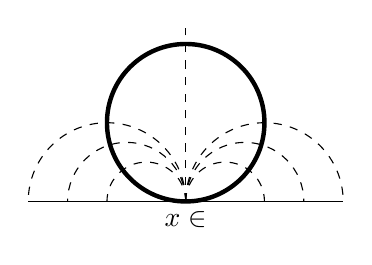
\begin{tikzpicture}[baseline=(X.base)]
	\coordinate (X) at (0,0);
	\draw (-2,0) -- (2,0);
	\draw[ultra thick] (0,1) circle[radius=1];
	\node at (0,0) [below] {$x \in \R$};

	\foreach \x in {0.5, 0.75, 1} {
		\draw[dashed] (0,0) arc (180:0:\x);
		\draw[dashed] (0,0) arc (0:180:\x); }
	\draw[dashed] (0,0) -- (0, 2.2);
\end{tikzpicture}\qquad
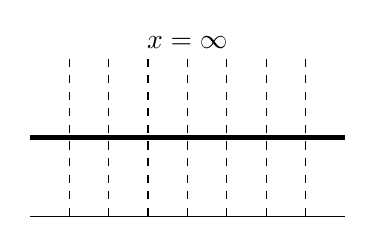
\begin{tikzpicture}[baseline=(X.base)]
	\coordinate (X) at (0,0);
	\draw (-2,0) -- (2,0);
	\draw[ultra thick] (-2,1) -- (2,1);
	\node at (0,2) [above] {$x=\infty$};

	\foreach \x in {-1.5, -1, -0.5, 0, 0.5, 1, 1.5}
		\draw[dashed] (\x, 0) -- (\x, 2);
\end{tikzpicture}
\end{center}
可以看出切点在 $x$ 的极限圆与全体过 $x$ 点的测地线族正交, 上图标为虚线. 从圆盘模型看得更清楚: 在 $\mathcal{D}$ 内部, 测地线无非是和 $\partial\mathcal{D} = \{z: |z|=1\}$ 正交的圆弧, 而极限圆正是内切 $\mathcal{D}$ 于一点的圆 (扣掉切点), 不必分开处理 $x = \infty$ 的情形.

\begin{definition}\label{def:geodesic-polygon} \index{cediduobianxing@测地多边形 (geodesic polygon)} \index{jiandian@尖点 (cusp)}
	上半平面 $\mathcal{H}$ 或圆盘模型 $\mathcal{D}$ 中的\emph{测地多边形}意指一个单连通的闭子集 $D$, 使得 $\partial D$ 由有限多条头尾相接的测地线段所围出; 依此可以谈论测地多边形的顶点 (即两边的接点) 及其内角. 这里容许顶点为\emph{尖点}, 也就是两条测地线在 $\R \sqcup \{\infty\}$ (上半平面) 或 $\{z: |z|=1 \}$ (圆盘模型) 中的交点.
	
	由于测地线总和边界正交, 尖点处的内角可以合理地定义为 $0$.
\end{definition}

回忆到双曲度量下的角度与标准度量 $|\dd\tau|^2$ 下无异. 圆盘模型中的尖点图像如下.
\begin{equation}\label{eqn:cusp-picture}\begin{tikzpicture}[scale=1.5, baseline=(B)]
	\fill[draw=white, shading=axis, top color=white, bottom color=gray!20] (1, 1.5) -- (1,1) arc(90:180:1) arc(0:90:1) -- (-1, 1.5) --cycle; 
	\draw[thick] (1,1) arc(90:180:1) arc(0:90:1);
	\draw[dashed] (1.5, 1.5) arc[start angle = 0, end angle=-180, radius=1.5];
	\node (B) at (0, 1) {$D$};
	\draw[fill=white] (0,0) circle[radius=1.2pt] node[below] {尖点};
	\node at (1.8, 0.8) {$|z|=1$};
\end{tikzpicture}\end{equation}
兹举 $\mathcal{H}$ 中一则反例, 下图不是测地多边形: 它由两条测地线围出, 但它们的头尾并未相接, 该区域朝边界 $\R \sqcup \{\infty\}$ 方向是``开''的.
\begin{center}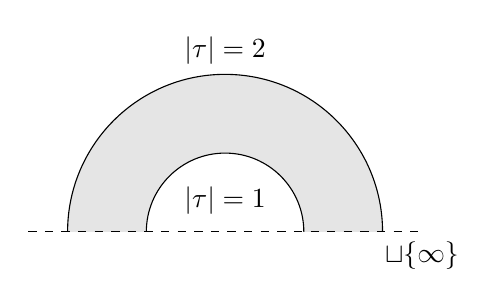
\begin{tikzpicture}
	\fill[color=gray!20] (-2, 0) arc(180:0:2) -- (1, 0) arc(0:180:1) --cycle;
	\draw (-2, 0) arc(180:0:2) node[midway, above, color=black] {$|\tau| = 2$};
	\draw (-1, 0) arc(180:0:1) node[midway, below=3mm, color=black] {$|\tau| = 1$};
	\draw[dashed] (-2.5, 0) -- (2.5, 0) node[below] {$\R \sqcup \{\infty\}$};
\end{tikzpicture}\end{center}

\begin{theorem}[Gauss--Bonnet 公式]\label{prop:Gauss-Bonnet} \index{Gauss--Bonnet 公式}
	设 $D$ 是测地多边形, 顶点为 $x_1, \ldots, x_n$ (容许尖点), 相应的内角为 $\alpha_1, \ldots, \alpha_n$ (容许 $\alpha_i = \pi$), 则相对于双曲度量的面积为
	\[ \mes(D) = (n-2)\pi - \sum_{i=1}^n \alpha_i. \]
\end{theorem}
\begin{proof}
	双曲度量的曲率为 $-1$. 因为 $D$ 单连通, 其 Euler 示性数是 $\chi = 1$. 如果 $\partial D$ 不含尖点, 则 $D$ 显然紧, 相应的结果无非是 Gauss--Bonnet 定理 \cite[附录一, \S 6]{ChCh}.
	
	含尖点的情形可以严谨地化约到上述情形, 想法是用截断来逼近. 我们逐一处理每个尖点附近的性状. 不失一般性可设 $D \subset \mathcal{H}$ 而该尖点为 $\infty$, 夹住尖点的两条测地线是 $\Re(\tau) = \pm\frac{1}{2}$, 引入截断参数 $M > 0$ 计算如下:
	\begin{center}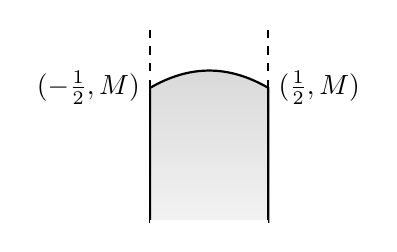
\begin{tikzpicture}[scale=1.5]
		\filldraw[thick, shading=axis, top color=gray!30, bottom color=gray!10] (120:1) -- (-0.5, 2) node [left] {$(-\frac{1}{2}, M)$} to [bend left] (0.5, 2) node [right] {$(\frac{1}{2}, M)$} -- (60:1) --cycle;
		\draw[ultra thick, white] (60:1) -- (120:1);
		\draw[thick, dashed] (-0.5, 2) -- (-0.5, 2.5);
		\draw[thick, dashed] (0.5, 2) -- (0.5, 2.5);
	\end{tikzpicture}\end{center}
	其中顶部曲线是测地线. 截断后 $D$ 的顶点数 $+1$. 另一方面, 当 $M \to +\infty$ 时, 顶部测地线趋于水平, 新添的顶点其内角和趋近于 $\frac{\pi}{2} + \frac{\pi}{2} = \pi$; 代入不含尖点的 Gauss--Bonnet 公式并取极限, 便出断言的答案. 
\end{proof}

\begin{corollary}\label{prop:angle-defect}
	任何测地三角形 $\Delta$ 的内角 $\alpha, \beta, \gamma$ 都满足 $\alpha + \beta = \pi - \gamma - \mes(\Delta)$.
\end{corollary}

\section{变换的分类和不动点}\label{sec:fixed-points}
我们在 \S\ref{sec:linear-fractional-transform} 已经看到, $\gamma = \twomatrix{a}{b}{c}{d} \in \GL(2,\R)$ 在 $\CC \sqcup \{\infty\}$ 上的作用相当于它在 $\PP^1(\CC) := \{ \text{直线}\; \subset \CC^2 \}$ 上的自然作用. 解不动点相当于解特征向量, 第一步则是解特征方程式 $\lambda^2 - \Tr(\gamma)\lambda + \det\gamma = 0$, 其判别式为 $\Tr(\gamma)^2 - 4\det\gamma$. 实根给出 $\R^2$ 中的特征向量, 相异根给出线性无关的特征向量; 重根情形下, 有一对线性无关的特征向量当且仅当 $\gamma$ 是纯量矩阵.

\begin{definition}\label{def:classification-matrices} \index{paowuyuan@抛物元 (parabolic element)} \index{tuoyuanyuan@椭圆元 (elliptic element)} \index{shuangquyuan@双曲元 (hyperbolic element)}
	称非纯量矩阵 $\gamma \in \GL(2,\R)^+$ 是
	\begin{itemize}
		\item \emph{椭圆}的, 如果 $\Tr(\gamma)^2 < 4\det\gamma$, 这时在它 $\mathcal{H}$ 中恰有一个不动点, 另一个不动点则为其复共轭, 属于 $-\mathcal{H}$;
		\item \emph{抛物}的, 如果 $\Tr(\gamma)^2 = 4\det\gamma$, 这时它恰有一个不动点, 落在 $\R \sqcup \{\infty\}$ 上;
		\item \emph{双曲}的, 如果 $\Tr(\gamma)^2 > 4\det\gamma$, 这时它有在 $\R \sqcup \{\infty\}$ 上有两个相异不动点.
	\end{itemize}
	这些性质只和 $\gamma$ 在 $\PGL(2,\R) \smallsetminus \{1\}$ 中的像有关.
\end{definition}

我们主要着眼于 $\gamma \in \SL(2,\R)$ 的情况. 因为 $\SL(2,\R)$ 在 $\mathcal{H}$ 上可递, 在椭圆情形下取 $\gamma$ 的适当共轭, 可假设不动点就是 $i \in \mathcal{H}$, 那么必有 $\gamma \in \SO(2,\R)$, 从圆盘模型观照, $\gamma$ 无非是旋转. 在抛物情形下, 线性代数告诉我们 $\gamma$ 共轭于某个 $\pm\twomatrix{1}{h}{}{1}$, $h \in \R^\times$, 相应的变换是平移. 同样由线性代数知双曲情形下 $\gamma$ 共轭于某个 $\twomatrix{a}{}{}{a^{-1}}$, $a \neq \pm 1$, 相应的变换是 $\tau \mapsto a^2\tau$.

留意到若 $\gamma$ 是抛物元, 那么当 $n \neq 0$ 时, $\gamma^n$ 仍是抛物元.

\begin{exercise}
	严格来说, 线性代数只告诉我们在群 $\GL(2,\R)$ 里能对抛物和双曲变换取如是共轭, 请说明如何将之细化到 $\SL(2,\R)$ 中的共轭.

	\begin{hint}
		对任意 $\lambda \in \R^\times$ 取 $g := \twomatrix{1}{}{}{\lambda}$, 那么 $g \twomatrix{1}{h}{}{1} g^{-1} = \twomatrix{1}{h/\lambda}{}{1}$ 而 $g\twomatrix{a}{}{}{a^{-1}} g^{-1} = \twomatrix{a}{}{}{a^{-1}}$. 以此 $g$ 将所求的共轭改进到 $\SL(2, \R)$.
	\end{hint}
\end{exercise}

\begin{example}[双曲变换, 轴和不动点]\label{eg:sliding}
	若 $\gamma \in \PSL(2,\R)$ 是双曲元, 令 $\mathcal{A}$ 为连接它两个不动点的测地线, 称为 $\gamma$ 的轴, 则 $\gamma$ 共轭 $\mathcal{A}$ 到 $\mathcal{A}$ 的等距变换. 如将 $\gamma$ 对角化为 $\twomatrix{a}{}{}{a^{-1}}$, 立见它诱导 $\mathcal{A} = [0, \infty]$ 上的平移.
	
	以下则逆向考察保持测地线的变换. 设 $\mathcal{A}$ 为测地线, 以 $x,y$ 为无穷远处的两端. 若 $\gamma \in \PGL(2,\R)$ 在 $\mathcal{A}$ 上诱导等距变换, 则按照 $\mathcal{A} \simeq \R$ 上等距变换熟知的分类, 有两种可能.
	\begin{compactitem}
		\item 或者 $\gamma|_{\mathcal{A}}$ 是平移, 这时 $\gamma x = x$ 而 $\gamma y = y$, 特别地 $\gamma$ 或者是 $\identity$, 或者是双曲元.
		\item 或者 $\gamma|_{\mathcal{A}}$ 是对某一点 $\eta$ 的反射, 这时 $\gamma$ 交换 $x$, $y$ 而 $\gamma^2|_{\mathcal{A}} = \identity$; 因 $\gamma$ 是 $\mathcal{H}$ 上的全纯变换, 这蕴涵 $\gamma^2 = 1$, 从而 $\gamma$ 是二阶椭圆元. 如果将 $\eta$ 搬运到圆盘模型的原点, $\gamma$ 便化为角度 $\pi$ 的旋转.
	\end{compactitem}
	在双曲情形下, 不失一般性可设 $x=0$ 而 $y = \infty$. 取 $a > 0$ 使得 $2\log a$ 为 $\gamma|_{\mathcal{A}}$ 的平移步长, 那么 $\gamma$ 映三元组 $(0, i, \infty)$ 为 $(0, a^2 i, \infty)$; 交比理论说明这样的 $\gamma$ 唯一, 显式取法无非是
	\[ \gamma = \twobigmatrix{a}{}{}{a^{-1}}. \]
	我们顺带导出 $\gamma|_{\mathcal{A}} = \identity_{\mathcal{A}}$ 蕴涵 $\gamma = 1$.
	\begin{center}\begin{tikzpicture}
		[geod/.style={draw, thick, arrows = {-Latex[scale length=0.5] . Latex[scale length=0.5]}}]
		\draw[dashed] (-4, 0) -- (4, 0);
		\draw[geod] (-3, 0) node[below] {$x$} arc(180:2:1) node[midway, above] {$\mathcal{A}$} node[below] {$y$};
		\draw[geod] (2,0) arc (270:-88:0.7) node[below] {$x = y$};
		\node at (-2, -1) {测地线};
		\node at (2, -1) {极限圆};
	\end{tikzpicture}\end{center}
	当 $y$ 趋近于 $x$, 测地线 $\mathcal{A}$ 退化为切 $x$ 的极限圆. 映极限圆为自身的 $\gamma \in \PGL(2,\R)$ 或者平凡, 或者是以 $x$ 为唯一不动点的抛物元. 反之, 以 $x$ 为唯一不动点的抛物元也保持所有切 $x$ 的极限圆不变, 请读者动手验证 (不妨设 $x = \infty$).
\end{example}

接着将焦点转向椭圆元素.
\begin{example}\label{eg:Gamma1-neat}
	设 $\gamma \in \SL(2,\Z)$ 满足 $\gamma \equiv \twomatrix{1}{*}{}{1} \pmod{N}$, 其中 $N \in \Z_{\geq 1}$. 我们断言当 $N \geq 4$ 时 $\gamma$ 不可能是椭圆元素. 诚然, 将 $\gamma$ 写作 $\twomatrix{1 + uN}{*}{*}{1 + vN}$, 那么椭圆的定义相当于 $(2 + (u+v)N)^2 < 4$, 仅当 $2 + (u+v)N \in \{0, 1, -1\}$ 时方有可能, 这就导致 $N$ 必须整除 $2,1,3$ 其中之一.
\end{example}

\begin{exercise}\label{exo:Gamma-neat}
	如果 $N = 2,3$, 那么上述论证中 $u + v = -1$. 以此证明若 $\gamma \in \SL(2,\Z)$ 满足 $\gamma \equiv \twomatrix{1}{}{}{1} \pmod{N}$, 那么 $N \geq 2$ 时 $\gamma$ 不可能是椭圆元素.
\end{exercise}

\begin{definition}[椭圆点]\label{def:elliptic-point} \index{tuoyuandian@椭圆点 (elliptic point)}
	设 $\Gamma$ 是 $\SL(2,\R)$ 的离散子群. 若 $\overline{\Gamma}_\tau \neq \{1\}$ 则称 $\tau \in \mathcal{H}$ 是 $\overline{\Gamma}$ 或 $\Gamma$ 的椭圆点.
\end{definition}

由定义立见 $\tau$ 是 $\Gamma$ 的椭圆点当且仅当存在 $\Gamma$ 中的椭圆元素 $\gamma$, 使得 $\tau$ 是 $\gamma$ 在 $\mathcal{H}$ 上的唯一不动点. 此性质只和 $\tau$ 的 $\overline{\Gamma}$ 轨道相关.

\begin{lemma}\label{prop:elliptic-pt-discrete}
	对于任何离散子群 $\Gamma$, 其椭圆点都构成 $\mathcal{H}$ 的离散子集.
\end{lemma}
\begin{proof}
	离散子群 $\Gamma$ 在 $\mathcal{H}$ 上的作用总是正常 (命题 \ref{prop:discrete-group-discontinuous-SL}), 因此 $\mathcal{H}$ 有一组开覆盖, 使得其中每个开集 $U$ 皆有紧闭包 $\bar{U}$, 并且 $\Xi_U := \left\{ \gamma \in \overline{\Gamma}: \gamma\bar{U} \cap \bar{U} \neq \emptyset\right\}$ 有限. 这样的开集 $U$ 仅含有限个椭圆点, 这是因为 $\tau \in U$ 和 $\gamma\tau = \tau$ 蕴涵 $\gamma \in \Xi_U$, 而每个 $\gamma \in \Xi_U \smallsetminus \{1\}$ 在 $\mathcal{H}$ 上至多仅有一个不动点.
\end{proof}

我们需要一个广为人知的初等代数结果.
\begin{proposition}\label{prop:disc-subgroup-circle}
	加法群 $\R$ 的非平凡离散子群都 $\simeq \Z$. 设 $A$ 是 $\R/\Z$ 的离散子群, 则 $A$ 是有限循环群, 它形如 $\frac{1}{h}\Z/\Z$, $h \in \Z_{\geq 1}$.
\end{proposition}

注意到 $\R/\Z \rightiso \{z \in \CC^\times: |z|=1 \}$, 办法是 $a \mapsto e^{2\pi ia}$. 由此推知后者的离散子群皆形如 $\mu_h = \{z \in \CC^\times : z^h=1 \}$.

\begin{proof}
	设 $\tilde{A}$ 是 $\R$ 的非平凡离散子群. 存在正数 $\tilde{a} \in \tilde{A} \smallsetminus \{0\}$ 使 $\tilde{a}$ 极小, 那么熟知的带余除法技巧给出 $\tilde{A} = \Z\tilde{a}$.
	
	设 $A \subset \R/\Z$ 为离散子群, $\R/\Z$ 紧蕴涵 $A$ 有限. 其逆像 $\tilde{A} \subset \R$ 也离散, 故形如 $\Z\tilde{a}$. 从 $|A| \tilde{a} \subset \Z$ 可知 $\tilde{a}$ 是有理数, 表作既约分式 $k/h$. 因为存在 $m$ 使得 $mk \equiv 1 \pmod h$, 故 $\frac{1}{h} \bmod \Z$ 也是 $A$ 的生成元. 证毕.
\end{proof}

\begin{proposition}\label{prop:stabilizer-finite-cyclic}
	对任意离散子群 $\Gamma \subset \SL(2,\R)$ 和 $\gamma \in \overline{\Gamma} \smallsetminus \{1\}$, 以下陈述等价:
	\begin{compactenum}[(i)]
		\item $\gamma$ 在 $\mathcal{H}$ 上有不动点,
		\item $\gamma$ 是有限阶的,
		\item $\gamma$ 是椭圆的.
	\end{compactenum}
	此外, 对任意 $\tau \in \mathcal{H}$, 群 $\Gamma_\tau$ 总是有限循环群.
\end{proposition}
\begin{proof}
	(i) $\implies$ (ii): 子群 $K := \Stab_{\SL(2,\R)}(\tau)$ 在 $\tau = i$ 时等于 $\SO(2,\R)$, 因而对任意 $\tau \in \mathcal{H}$ 皆有 $K \simeq \SO(2,\R) \simeq \{z \in \CC^\times: |z|=1 \}$. 从命题 \ref{prop:disc-subgroup-circle} 可知 $K$ 的离散子群必为有限循环群, 其元素 $\gamma$ 当然有限阶. 这一并证明了 (ii) 和最后部分的断言.

	(ii) $\implies$ (iii): 有限阶元素 $\gamma$ 总能在 $\GL(2,\CC)$ 中对角化为 $\twomatrix{z}{}{}{z^{-1}}$ 之形, 其中 $z$ 是单位根. 如 $\gamma \neq \pm 1$ 则 $|\Tr(\gamma)| = |z + z^{-1}| = |z^2 + 1| < 2$.
	
	(iii) $\implies$ (i): 业已在定义 \ref{def:classification-matrices} 中说明.
\end{proof}

下述简单结果将在 \S\ref{sec:dimension-formula-odd} 用到.
\begin{proposition}\label{prop:elliptic-odd}
	设元素 $\gamma \in \Gamma$ 的阶数为偶数, 那么 $-1 \in \Gamma$.
	
	作为推论, 若 $-1 \notin \Gamma$, 则对所有 $\tau \in \mathcal{H}$, 群 $\overline{\Gamma}_\tau = \Gamma_\tau$ 的阶必为奇数.
\end{proposition}
\begin{proof}
	设 $\gamma$ 阶数为 $2a$. 在 $\GL(2, \CC)$ 中把 $\gamma$ 对角化为 $\twomatrix{z}{}{}{z^{-1}}$, 其中 $z \in \CC^\times$ 是 $2a$ 次本原单位根, $a \in \Z_{\geq 1}$. 因此 $\gamma^a = -1 \in \Gamma$. 这就证明了第一个断言.
	
	对于第二个断言, 条件蕴涵 $\Gamma = \overline{\Gamma}$. 我们知道 $\Gamma_\tau$ 是有限循环群. 其阶数若为偶数则与第一个断言矛盾.
\end{proof}


\section{同余子群, 尖点, 基本区域}\label{sec:cong-subgroup}
\begin{definition}
	\index{moqun@模群 (modular group)} \index{zhutongyuziqun@主同余子群 (principal congruence subgroup)} \index{ji@级 (level)}
	\index[sym1]{GammaN@$\Gamma(N)$, $\Gamma_1(N)$, $\Gamma_0(N)$}
	称 $\SL(2,\Z)$ 为\emph{模群}, 它自然地左作用于 $\mathcal{H}$ 上. 对于任意 $N \in \Z_{\geq 1}$, 定义
	\[\begin{tikzcd}[row sep=tiny, column sep=small]
		\Gamma(N) \arrow[r, phantom, ":=" description] \arrow[d, phantom, sloped, "\subset"] & \left\{ \gamma \in \SL(2,\Z) : \gamma \equiv \begin{pmatrix} 1 & \\ & 1 \end{pmatrix} \pmod N \right\}, \\
		\Gamma_1(N)  \arrow[r, phantom, ":=" description] \arrow[d, phantom, sloped, "\subset"] & \left\{ \gamma \in \SL(2,\Z) : \gamma \equiv \begin{pmatrix} 1 & * \\ & 1 \end{pmatrix} \pmod N \right\}, \\
		\Gamma_0(N)  \arrow[r, phantom, ":=" description] & \left\{ \gamma \in \SL(2,\Z) : \gamma \equiv \begin{pmatrix} * & * \\ & * \end{pmatrix} \pmod N \right\}.
	\end{tikzcd}\]
	称 $\Gamma(N)$ 为 $N$ 级的\emph{主同余子群}.
\end{definition}

留意到 $\Gamma(1) = \SL(2,\Z)$, 此外 $\Gamma(N) = \Ker\left[ \SL(2,\Z) \xrightarrow{\bmod N} \SL(2,\Z/N\Z) \right]$, 而 $N' \mid N$ 蕴涵 $\Gamma(N) \lhd \Gamma(N')$.

\begin{exercise}
	证明 $\Gamma_1(N) \lhd \Gamma_0(N)$, 而 $\twomatrix{a}{b}{c}{d} \mapsto d \bmod N$ 给出同构 $\Gamma_0(N)/\Gamma_1(N) \simeq (\Z/N\Z)^\times$.
\end{exercise}

\begin{definition}\index{tongyuziqun@同余子群 (congruence subgroup)}
	设 $\Gamma$ 为 $\SL(2,\Z)$ 的子群. 若存在 $N$ 使得 $\Gamma \supset \Gamma(N)$, 则称 $\Gamma$ 为 $\SL(2,\Z)$ 的\emph{同余子群}.
\end{definition}

观察到同余子群总是 $\SL(2,\R)$ 的离散子群, 证明 $\SL(2,\Z)$ 是离散子群即可: 这是因为 $\SL(2,\R)$ 的拓扑来自于嵌入 $\SL(2,\R) \hookrightarrow \Mat_2(\R)$; 显然 $\Mat_2(\Z)$ 在 $\Mat_2(\R)$ 中离散, 而 $\Mat_2(\Z) \cap \SL(2, \R) = \SL(2, \Z)$.

此外, 同余子群 $\Gamma$ 必满足 $(\SL(2, \Z): \Gamma)$ 有限. 这是因为 $\Gamma \supset \Gamma(N)$ 导致
\[ (\SL(2, \Z): \Gamma) \;\text{整除}\; (\SL(2, \Z): \Gamma(N)) = \left| \Image\left[ \SL(2, \Z) \xrightarrow{\bmod N} \SL(2, \Z/N\Z) \right] \right|, \]
末项当然有限. 以下说明 $\bmod\; N$ 实际还是满射, 此性质将反复应用.

\begin{proposition}\label{prop:reduction-surjective}
	对任意 $N$, 由 $\Z \twoheadrightarrow \Z/N\Z$ 诱导的同态 $\SL(2,\Z) \xrightarrow{\bmod N} \SL(2, \Z/N\Z)$ 是满的. 作为推论, $(\SL(2,\Z):\Gamma(N)) = |\SL(2, \Z/N\Z)|$.
\end{proposition}
\begin{proof}
	设 $\bar{a}, \bar{b}, \bar{c}, \bar{d} \in \Z/N\Z$ 满足 $\bar{a}\bar{d}-\bar{b}\bar{c}=1$. 今求代表元 $a,b,c,d \in \Z$ 使得 $ad-bc=1$. 从任取之代表元 $a,b,c,d$ 出发, 依序论证
	\begin{compactitem}
		\item $\gcd(a,b)$ 和 $\gcd(c,d)$ 皆与 $N$ 互素;
		\item 可修改 $a,b$ 使之互素: 先考虑 $a \neq 0$ 情形, 以 $b+tN$ 代 $b$, 其中
			\[ t \equiv \begin{cases}
				1 \pmod p, & \forall\; \text{素数}\; p \mid \gcd(a,b) \\
				0 \pmod p, & \forall\; \text{素数}\; p \nmid \gcd(a,b), \; p \mid a
			\end{cases} \]
			继而对任意素数 $p$ 验证 $p \mid a \implies p \nmid b + tN$; 如果 $b \neq 0$, 在论证中对调 $a,b$ 即可;
		\item 取定互素之 $a,b$, 存在 $u,v \in \Z$ 满足
		\[ av - bu = \frac{1 - (ad-bc)}{N}, \]
		以 $c + uN$ 和 $d + vN$ 取代 $c$ 和 $d$, 即可确保 $ad - bc=1$.
	\end{compactitem}
	这些论证无非是初等数论.
\end{proof}

行将定义的模形式与商空间 $\Gamma \backslash \mathcal{H}$ 的几何有极密切的联系. 几何工具在非紧空间上不易施展, 是以此处的关键在于向 $\Gamma \backslash \mathcal{H}$ 添入一些\emph{尖点}予以紧化. 本节先就同余子群情形探讨尖点的群论面向, 稍后的 \S\ref{sec:Dirichlet-domain} 则探究双曲几何面向, 两者当然是关连的.

先前已说明 $\SL(2,\R)$ 在 $\CC \sqcup \{\infty\}$ 上的作用保持 $\mathcal{H}$ 及其边界 $\partial\mathcal{H} = \R \sqcup \{\infty\}$. 探讨同余子群的尖点时, 考虑子集 $\Q^* := \Q \sqcup \{\infty\}$ 便已足够. 群 $\SL(2,\Q)$ 保持 $\Q^*$, 因而 $\SL(2,\Z)$ 亦然. 将 $\Q^* \simeq \PP^1(\Q)$ 的元素以齐次坐标表作 $(x:y)$ 之形. 那么 $\SL(2,\Z)$ 的作用无非是
\[ \begin{pmatrix} a & b \\ c & d \end{pmatrix} (x:y) = (ax+by:cx+dy), \quad (x, y) \in \Z^2 \smallsetminus \{(0, 0)\}. \]
通分后不妨设以上之 $x, y \in \Z$ 互素.

\begin{definition}\label{def:cusp-congruence-subgroup} \index{jiandian}
	一个同余子群 $\Gamma$ 的\emph{尖点}定为 $\Q^*$ 在 $\Gamma$ 作用下的等价类.
\end{definition}

\begin{proposition}\label{prop:cusp-finiteness}
	模群 $\SL(2,\Z)$ 恰有一个尖点 $\infty$. 任意同余子群 $\Gamma$ 都只有有限多个尖点.
\end{proposition}
\begin{proof}
	先处理 $\SL(2,\Z)$. 仅须说明对所有互素的 $a,c \in \Z$, 皆存在 $\gamma \in \SL(2,\Z)$ 使得 $\gamma(1:0) = (a:c)$. 诚然, 存在 $b,d \in \Z$ 使得 $ad - bc = 1$, 取 $\gamma = \bigl(\begin{smallmatrix} a & b \\ c & d \end{smallmatrix} \bigr)$ 即是.

	给定同余子群 $\Gamma$, 存在 $k \in \Z_{\geq 1}$ 和 $g_1, \ldots, g_k$ 使得 $\SL(2,\Z) = \bigsqcup_{i=1}^k \Gamma g_i$, 因此 $\Q^* = \SL(2,\Z)\infty = \bigcup_{i=1}^k \Gamma g_i \infty$.
\end{proof}

引理 \ref{prop:stab-cusp} 的立即推论是 $\Stab_{\PSL(2,\Z)}(\infty) = \twomatrix{1}{*}{}{1}$, 因为 $\SL(2,\Z)$ 中的上三角矩阵其对角元必为 $\pm 1$.

今后的论证中经常需要控制某个 $\tau \in \mathcal{H}$ 在同余子群作用下的轨道, 以下引理是一个有效工具.
\begin{lemma}\label{prop:finiteness-aux}
	设 $K \subset \mathcal{H}$ 是紧子集, 则对于任何 $t \in \R_{>0}$, 集合
	\[ \left\{ (c,d) \in \R^2 : \exists \gamma = \twomatrix{a}{b}{c}{d} \in \SL(2, \R), \; \tau \in K, \; \Im(\gamma\tau) \geq t \right\} \]
	在 $\R^2$ 中有界.
\end{lemma}
\begin{proof}
	当 $\tau \in \mathcal{H}$ 固定, 函数 $(c,d) \mapsto |c\tau+d|^2$ 是 $\R^2$ 上的正定二次型, 它对 $\tau$ 连续地变化, 因之可选取 $\tau$ 的连续函数 $m(\tau) > 0$ 使得
	\[ m(\tau) \leq \dfrac{ |c\tau + d|^2 }{ \max\{ |c|, |d| \}^2 }, \quad (c,d) \in \R^2. \]
	根据引理 \ref{prop:fractional-transform-sign}, 若 $\gamma = \twomatrix{a}{b}{c}{d}$ 则
	\[ \Im(\gamma \tau) = |c\tau+d|^{-2} \Im(\tau) \leq m(\tau)^{-1} \Im(\tau) \max\{ |c|, |d| \}^{-2}. \]
	既然 $K$ 紧, 条件 $\Im(\gamma\tau) \geq t$ 和 $\tau \in K$ 遂给出上界
	\[ \max\{|c|, |d|\}^2 \leq t^{-1} \underbracket{\max_{\tau \in K} \left( m(\tau)^{-1} \Im(\tau) \right)}_{\in \R_{>0}}. \]
	明所欲证.
\end{proof}

\begin{exercise}
	试以引理 \ref{prop:finiteness-aux} 直接证明 $\SL(2,\Z)$ 在 $\mathcal{H}$ 上的作用是正常的 (参看命题 \ref{prop:discrete-group-discontinuous-SL}), 不依赖命题 \ref{prop:discrete-group-discontinuous}.
\end{exercise}

命题 \ref{prop:discrete-group-discontinuous-SL} 已经说明 $\SL(2,\R)$ 的离散子群在 $\mathcal{H}$ 上正常地作用, 这就启发我们探究同余子群 $\Gamma$ 或 $\overline{\Gamma}$ 的基本区域, 见定义 \ref{def:fundamental-domain}. 且先从 $\Gamma = \SL(2,\Z)$ 起步. 定义闭集 \index{jibenquyu@基本区域 (fundamental domain)}
\begin{equation}\label{eqn:fundamental-domain-full}
	\mathcal{F} := \left\{ \tau \in \mathcal{H}: -\frac{1}{2} \leq \Re(\tau) \leq \frac{1}{2}, \; |\tau| \geq 1 \right\}.
\end{equation}
\begin{center}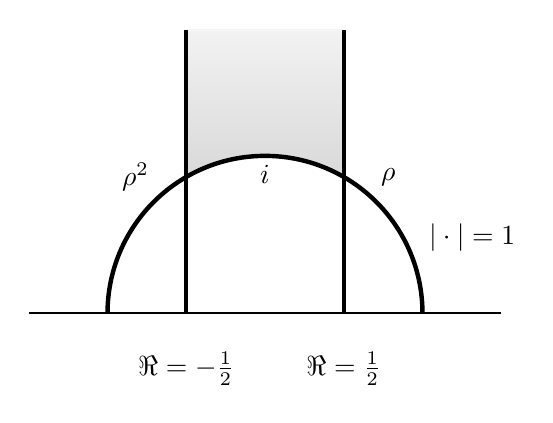
\begin{tikzpicture}[scale=2]
	\fill[draw=white, shading=axis, bottom color=gray!30, top color=gray!10] (-0.5, 1.8) -- (120:1) node [left=1em, color=black] {$\rho^2$} arc(120:60:1) node [right=1em, color=black] {$\rho$} -- (0.5, 1.8) --cycle;
	\draw[ultra thick] (-0.5, 1.8) -- (-0.5, 0) node [below=1em] {$\Re= -\frac{1}{2}$};
	\draw[ultra thick] (0.5, 1.8) -- (0.5, 0) node [below=1em] {$\Re= \frac{1}{2}$};
	\draw[ultra thick] (1, 0) arc(0:180:1);
	\node at (0,1) [below] {$i$};
	\draw[thick] (-1.5, 0) -- (1.5, 0);
	\node at (20: 1.4) {$|\cdot|=1$};
\end{tikzpicture}\end{center}
很显然, $\mathcal{F}$ 的右左两角分别是 \index[sym1]{rho@$\rho$}
\[ \rho := \frac{1}{2} + \frac{\sqrt{-3}}{2} = e^{2\pi i/6},  \quad \rho^2 = \frac{-1}{2} + \frac{\sqrt{-3}}{2}. \]
应该理解 $\mathcal{F}$ 为三条测地线围出的一个\emph{测地三角形} (定义 \ref{def:geodesic-polygon}), 以 $\rho, \rho^2, \infty$ 为顶点, 两条垂直测地线相切于 $\infty$, 而 $\infty$ 也是 $\SL(2,\Z)$ 的唯一尖点之代表元.

\begin{lemma}\label{prop:full-fundamental-domain-aux}
	设 $\tau_1, \tau_2 \in \mathcal{F}$, 存在 $\gamma \in \SL(2,\Z)$ 使得 $\gamma \tau_1 = \tau_2$ 当且仅当以下任一条件成立:
	\begin{compactitem}
		\item $\tau_1 = \tau_2$, 或
		\item $\Re(\tau_1) = \pm \frac{1}{2}$, $\tau_2 = \tau_1 \mp 1$, 或
		\item $|\tau_1|=1$, $\tau_2 = -1/\tau_1$.
	\end{compactitem}
	若 $\tau_1$ 或 $\tau_2$ 属于 $\mathcal{F}^\circ$, 则 $\gamma\tau_1 = \tau_2$ 成立当且仅当 $\gamma$ 在 $\PSL(2,\Z)$ 中的像平凡.
\end{lemma}
\begin{proof}
	记下一个平凡的观察: 令 $\mathcal{C} := \{z \in \CC: |z| \leq 1 \}$. 端详图形可知对于 $h \in \Z$,
	\[ \mathcal{F} \cap (h +  \mathcal{C} ) = \begin{cases}
		\left\{ \tau \in \mathcal{H}: |\tau| = 1, \; \frac{1}{2} \leq \Re(\tau) \leq \frac{1}{2} \right\}, & h=0, \\
		\{\rho\}, & h = 1, \\
		\{\rho^2 \}, & h = -1, \\
		\emptyset, & |h| > 1.
	\end{cases}\]
	继而设 $\tau_1 = x+iy \in \mathcal{F}$, $\tau_2 = \gamma\tau_1 \in \mathcal{F}$, 其中 $\gamma = \bigl(\begin{smallmatrix} a & b \\ c & d \end{smallmatrix}\bigr) \in \SL(2,\Z)$. 不妨设 $\Im(\tau_1) \leq \Im(\tau_2)$. 引理 \ref{prop:fractional-transform-sign} 蕴涵 $|c\tau_1 + d|^2 = (cx+d)^2 + (cy^2) \leq 1$. 观察到 $y \geq \frac{\sqrt{3}}{2}$, 故必然有 $c = -1, 0, 1$.
	\begin{enumerate}[A.]
		\item 当 $c=0$ 时, $\gamma = \pm \bigl(\begin{smallmatrix} 1 & k \\ & 1 \end{smallmatrix}\bigr)$, 其中 $|k| \leq 1$, 此时或者 $\Re(\tau_1) = \pm \frac{1}{2}$ 而 $k=\mp 1$, 或者 $\tau_1=\tau_2$ 而 $k=0$.
		\item 当 $c=1$ 时我们得到 $|\tau_1 + d|^2 \leq 1$, 或者说 $\tau_1 \in \mathcal{F} \cap \left( -d + \mathcal{C} \right)$. 于是 $|d| \leq 1$, 而且 $d=\pm 1 \implies \tau_1 \in \{\rho, \rho^2\}$. 继续细分如下.
		\begin{compactitem}
			\item 当 $d=0$ 时 $|\tau_1|=1$, $\gamma = \bigl(\begin{smallmatrix} a & -1 \\ 1 & 0 \end{smallmatrix}\bigr)$ 的作用为 $\tau \mapsto a - \frac{1}{\tau}$. 这表明 $\tau_2 \in \mathcal{F} \cap \left(a + \mathcal{C} \right)$, 故 $|a| \leq 1$; 若 $a=0$ 则 $\tau_2 = -1/\tau_1$. 若 $a = \pm 1$ 则 $\tau_2 \in \{\rho, \rho^2\}$, 这时从 $-1/\tau_1 = \tau_2 \mp 1 \in \mathcal{F}$ 可算出唯二可能是
			\[ \tau_2 = \rho = \tau_1, \; a = +1, \quad \text{或} \quad \tau_2 = \rho^2 = \tau_1, \; a = -1. \]
			\item 当 $d=1$ 时, $|\tau_1 + 1| \leq 1$ 和 $\tau_1 \in \{ \rho, \rho^2\}$ 蕴涵 $\tau_1 = \rho^2$; 此时 $|\tau_1 + 1| = |\rho^2 + 1| = 1$ 导致 $\Im(\tau_2) = \Im(\tau_1)$ (引理 \ref{prop:fractional-transform-sign}), 故 $\tau_2 \in \{\rho, \rho^2\}$.
			\item 对于 $d=-1$ 可以类似地分析: 此时 $\tau_1 = \rho$ 而 $\tau_2 \in \{\rho, \rho^2\}$.
		\end{compactitem}
		\item 当 $c=-1$ 时, 以 $-\gamma$ 代 $\gamma$ 化约到情形 B.
	\end{enumerate}
	留意到当 $\tau_1$ 或 $\tau_2$ 属于 $\mathcal{F}^\circ$ 时,仅情形 A 的 $k=0$ 情形可能发生, 即 $\gamma = \pm 1$.
\end{proof}

上半平面的自同构 $\tau \mapsto -\frac{1}{\tau}$ 和 $\tau \mapsto \tau + 1$ 分别由 $\SL(2, \Z)$ 的下述元素给出
\begin{equation}\label{eqn:S-T}
	S := \begin{pmatrix} & -1 \\ 1 & \end{pmatrix}, \quad T := \begin{pmatrix} 1 & 1 \\ & 1 \end{pmatrix}; \quad S^2 = (ST)^3 = -1.
\end{equation}
观察到 $S$ 的作用无非是先反演, 再对虚轴镜射, 如下所示.
\begin{center}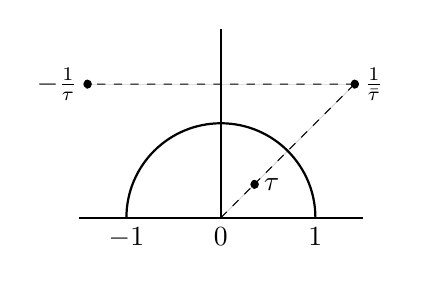
\begin{tikzpicture}[scale=1.2]
	\draw[thick] (1, 0) node[below] {$1$} arc(0:180:1) node[below] {$-1$};
	\draw[thick] (0, 2) -- (0, 0) node[below] {$0$};
	\draw[thick] (-1.5, 0) -- (1.5, 0);
	\filldraw[dashed] (0, 0) -- (45:0.5) circle[radius=1.2pt] node[right] {$\tau$}
		-- (45:2) circle[radius=1.2pt] node[right] {$\frac{1}{\bar{\tau}}$}
		-- (135:2) circle[radius=1.2pt] node[left] {$-\frac{1}{\tau}$};
\end{tikzpicture}\end{center}

\begin{theorem}\label{prop:full-fundamental-domain}
	定义于 \eqref{eqn:fundamental-domain-full} 的测地三角形 $\mathcal{F}$ 是 $\PSL(2,\Z)$ 在 $\mathcal{H}$ 上作用的一个基本区域, 而 $S, T$ 生成  $\SL(2,\Z)$.
\end{theorem}
\begin{proof}
	显然 $\mathcal{F}$ 是 $\mathcal{F}^\circ$ 的闭包, 故定义 \ref{def:fundamental-domain} 的 \textbf{F.1} 成立. 现在验证 \textbf{F.2} 所要求的 $\gamma, \gamma' \in \SL(2,\Z)$ 而 $\gamma \neq \pm\gamma'$ 蕴涵 $\gamma\mathcal{F}^\circ \cap \gamma'\mathcal{F}^\circ = \emptyset$: 不失一般性设 $\gamma' = 1$, 再应用引理 \ref{prop:full-fundamental-domain-aux} 即可.

	接着论证 $\bigcup_\gamma \gamma\mathcal{F}$ 局部有限. 给定 $\tau$, 取开邻域 $U \ni \tau$ 使闭包 $K := \bar{U}$ 为紧. 若$\gamma^{-1} K \cap \mathcal{F} \neq \emptyset$, 则存在 $\tau \in K$ 使得 $\Im(\gamma^{-1}\tau) \geq \sqrt{3}/2$, 故根据引理 \ref{prop:finiteness-aux}, $\gamma^{-1}$ 的第二行被控制在 $\Z^2$ 的一个有界子集中, 因而仅有有限种选取. 因为 $K$ 紧, 引理 \ref{prop:fractional-transform-sign} 对这样的 $\gamma$ 控制了 $\{ \Im(\gamma^{-1}\tau) : \tau \in K \}$: 它有一致的上界 $B$. 置 $\mathcal{F}' := \mathcal{F} \cap \{\Im \leq B \}$, 原条件化为 $\gamma^{-1} K \cap \mathcal{F}' \neq \emptyset$. 然而 $\mathcal{F}'$ 和 $K$ 皆紧, 命题 \ref{prop:discrete-group-discontinuous-SL} 遂蕴涵 $\gamma$ 的选取有限.

	下面证明 $\mathcal{H} = \bigcup_\gamma \gamma\mathcal{F}$. 老方法: 对取定的 $\tau \in \mathcal{H}$ 和任意 $t > 0$, 由引理 \ref{prop:finiteness-aux} (取 $K = \{\tau\}$) 可知满足 $\Im(\gamma\tau) \geq t$ 的 $\gamma \in \SL(2,\Z)$ 其第二行 $(c,d)$ 被控制在 $\Z^2$ 的有界子集中, 故选择有限. 结合引理 \ref{prop:fractional-transform-sign} 遂推得
	\[ \left\{ \Im(\gamma\tau) : \gamma \in \SL(2,\Z), \; \Im(\gamma\tau) \geq t \right\} \; \text{是有限集}. \]
	定义 $\Gamma^\flat$ 为 $S, T$ 在 $\SL(2,\Z)$ 中生成的子群. 以上观察确保在轨道 $\Gamma^\flat \tau$ 中可取 $\eta$ 使得 $\Im(\eta)$ 极大. 用 $T$ 左右平移来确保 $-\frac{1}{2} \leq \Re(\eta) \leq \frac{1}{2}$. 如果 $|\eta| \geq 1$ 则 $\eta \in \mathcal{F}$, 否则根据 $S$ 的直观性质将有 $\Im(S\eta) > \Im(\eta)$, 这与 $\eta$ 的选取矛盾. 由此确立 \textbf{F.3}.

	最后证明 $\Gamma^\flat = \SL(2,\Z)$, 对任意 $\gamma \in \SL(2,\Z)$, 取 $\tau \in (\gamma\mathcal{F})^\circ = \gamma\mathcal{F}^\circ$. 上段已论证存在 $\gamma^\flat \in \Gamma^\flat$ 使得 $\tau \in \gamma^\flat \mathcal{F}$, 从 $\gamma \mathcal{F}^\circ \cap \gamma^\flat \mathcal{F} \neq \emptyset$ 和内点的定义导出 $\gamma \mathcal{F}^\circ \cap \gamma^\flat \mathcal{F}^\circ \neq \emptyset$, 继而有 $\gamma = \pm \gamma^\flat$, 然而 $\pm 1 \in \Gamma^\flat$.
\end{proof}

上述结果蕴涵 $\SL(2,\Z)$ 的元素都可以表作 $T^{a_n} S T^{a_{n-1}} \cdots ST^{a_1}$, 其中 $a_1, \ldots, a_n \in \Z$. 从 $S,T$ 的作用方式立见
\[ T^{a_n} \cdots ST^{a_1}(\tau) =
	a_n - \cfrac{1}{ a_{n-1} -
		\cfrac{1}{a_{n-2} - \cdots
			\cfrac{1}{a_3 -
				\cfrac{1}{a_2 - \cfrac{1}{a_1
					+ \tau}
				}
			}
		}
	}
\]
其中 $\tau \in \CC \sqcup \{\infty\}$; 这也可以按经典的连分数理论来理解.

\begin{proposition}\label{prop:hyperbolic-volume}
	相对于双曲度量, $\mes(\mathcal{F}) = \frac{\pi}{3}$.
\end{proposition}
\begin{proof}
	易见顶点 $\rho, \rho^2, \infty$ 的内角分别是 $\frac{\pi}{3}$, $\frac{\pi}{3}$ 和 $0$, 应用定理 \ref{prop:Gauss-Bonnet} 即可.
\end{proof}

\begin{proposition}\label{prop:elliptic-pt-cyclic}
	精确到 $\SL(2,\Z)$-轨道, 模群 $\SL(2,\Z)$ 的椭圆点仅有 $i$ 和 $\rho := e^{2\pi i/6}$, 稳定化子群分别是
	\[ \Stab_{\SL(2,\Z)}(i) = \lrangle{ \twomatrix{}{-1}{1}{} }, \quad \Stab_{\SL(2,\Z)}(\rho) = \lrangle{ \twomatrix{}{-1}{1}{-1} },  \]
	它们在 $\PSL(2,\Z)$ 中的阶数分别是 $2$ 和 $3$. 对于一般的同余子群 $\Gamma \subset \SL(2,\Z)$, 相应的椭圆点集是有限个 $\Gamma$-轨道的并.
\end{proposition}
\begin{proof}
	在 $\mathcal{F}$ 中考虑即足. 相关计算已在引理 \ref{prop:full-fundamental-domain-aux} 的情形 B 中完成 (取 $\tau_1 = \tau_2$), 关于阶数的计算则是直截了当的, 留给读者作为练习.
	
	对于同余子群 $\Gamma$, 其椭圆点必然也是 $\SL(2,\Z)$ 的椭圆点, 而每一条 $\SL(2,\Z)$ 轨道都分解为有限多个 $\Gamma$ 轨道. 证毕.
\end{proof}

对于一般的同余子群 $\Gamma$, 取定陪集分解 $\PSL(2,\Z) = \bigsqcup_{i=1}^k \overline{\Gamma} g_i$. 在命题 \ref{prop:fundamental-domain-sub} 中代入 $\mathcal{F}$, $\PSL(2,\Z)$ 及其子群 $\overline{\Gamma}$ 就能得到其基本区域 $\mathcal{F}_\Gamma = \bigcup_{i=1}^k g_i\mathcal{F}$, 它的面积为 $k\pi/3$. 此构造还蕴涵 $\mathcal{F}_\Gamma$ 的``无穷远点'', 亦即它在 $\R \sqcup \{\infty\}$ 上的极限点组成了集合 $\left\{ g_i \infty : 1 \leq i \leq k \right\}$. 基于引理 \ref{prop:cusp-finiteness}, $\Gamma$ 的每个尖点都有形如 $g_i \infty$ 的代表元; 由于 $\mathcal{F}_\Gamma$ 在 $g_i \infty$ 附近的样貌正好是直观意义的``尖点'', 由此不难对定义 \ref{def:cusp-congruence-subgroup} 的内涵有最初步的领略.

基本区域的一般构造方式将在 \S\ref{sec:Dirichlet-domain} 介绍.

基本区域的取法并不唯一. 取 $\Gamma = \SL(2,\Z)$ 和如上的 $\mathcal{F}$ 为例, 可行如下操作.
\begin{compactenum}
	\item 将 $\mathcal{F}$ 沿虚数轴切成两个测地三角形, 左右两半分别标为灰白:
	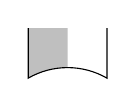
\begin{tikzpicture}[baseline=(C.center)]
		\fill[color=lightgray] (0, 1.5) -- (0,1) arc(90:120:1) -- (-0.5, 1.5) --cycle;
		\draw (-0.5, 1.5) -- (120:1) arc(120:60:1) -- (0.5, 1.5);
		\coordinate (C) at (0, 1);
	\end{tikzpicture}
%	这相当于向 $\overline{\Gamma}$ 添入对虚数轴的镜射 $r: \tau \mapsto -\bar{\tau}$, 得到的新变换群同构于 $\overline{\Gamma}' = \overline{\Gamma} \rtimes \{\identity, r\}$; 此处半直积由
%	\[ r \longmapsto [\gamma \mapsto {}^t \gamma^{-1} ] \in \Aut(\overline{\Gamma}) \]
%	定义 (思之). 群 $\overline{\Gamma}'$ 的基本区域可以取为任何一半.
	\item 因为 $\mathcal{F}$ 是基本区域, 这两半在 $\Gamma$ 作用下的所有像铺满 $\mathcal{H}$, 仍按灰白着色, 一般称之为 Dedekind 镶嵌. 譬如 $\mathcal{F}$ 对 $S$ 的像形如:
	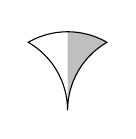
\begin{tikzpicture}[baseline=(C.center)]
		\fill[color=lightgray] (0, 0) -- (0,1) arc(90:60:1) arc(120:180:1);
		\draw (0,0) arc(0:60:1) arc(120:60:1) arc(120:180:1);
		\coordinate (C) at (0, 0.5);
\end{tikzpicture}
	\item 在 Dedekind 镶嵌中任取一个灰区并上一个白区, 皆是 $\Gamma$ 的基本区域. 例如:
		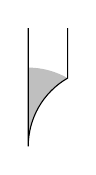
\begin{tikzpicture}[baseline=(C.center)]
			\fill[color=lightgray] (0,0) -- (0,1) arc(90:60:1) arc(120:180:1);
			\draw (0,1.5) -- (0,0) arc(180:120:1) -- (0.5, 1.5);
			\coordinate (C) at (0, 0.6);
		\end{tikzpicture}
\end{compactenum}

\begin{example}
	当 $\Gamma$ 为同余子群时, 已有算法能从 Dedekind 镶嵌中萃取 $\Gamma$ 的连通基本区域, 以下是软件求得 $\Gamma = \Gamma(7)$ 的结果, 算法给出一个宽度为 7 的基本区域, 无椭圆点, 计有 24 个尖点
	\[ 0, \frac{2}{7}, \frac{1}{3}, \frac{3}{7}, \frac{1}{2}, \frac{2}{3}, 1, \frac{4}{3}, \frac{3}{2}, \frac{5}{3}, 2, \frac{7}{3}, \frac{5}{2}, 3, \frac{10}{3}, \frac{7}{2}, 4, \frac{13}{3}, \frac{9}{2}, 5, \frac{11}{2}, 6, \frac{13}{2}, \infty. \]

	\begin{figure}[h]
		\centering
		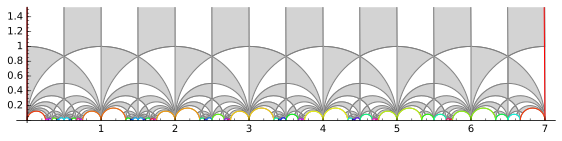
\includegraphics[width=\textwidth]{X7.png}
		\caption{$\Gamma(7)$ 的一个基本区域}
	\end{figure}
	添入这些尖点后得到一个耐人寻味的紧 Riemann 曲面, 亏格为 $3$ (例 \ref{eg:GammaN-genus}); 一旦充分掌握了模形式的知识, 可以证明它同构于所谓的 Klein 四次复射影曲线 (见 \cite[III.6]{KF1})
	\[ C_4 = \left\{ (x:y:z) \in \PP^2(\CC) : x^3 z + yz^3 + xy^3 = 0 \right\}; \]
	现代视角的讨论见 \cite[\S 4]{El99}. 这种\emph{紧化}的程序在 \S\ref{sec:X-charts} 将有进一步的讨论.
\end{example}

最后, 观察到以上构造的 $\mathcal{F}_\Gamma$ 其边界总是零测集. 关于基本区域的一个简单性质 (注记 \ref{rem:fundamental-domain-vol}) 表明测度 $\mes(\Gamma \backslash \mathcal{H})$ 无关 $\mathcal{F}_\Gamma$ 的选取, 它是 $\Gamma$ 的不变量.

\begin{exercise}\label{exo:congruence-order}
	对所有正整数 $N$, 证明
	\begin{align*}
		\left( \SL(2,\Z) : \Gamma(N) \right) & = N^3 \prod_{\substack{p: \text{素数} \\ p \mid N }} \left( 1 - \frac{1}{p^2} \right), \\
		\left( \SL(2,\Z) : \Gamma_1(N) \right) & = N^2 \prod_{\substack{p: \text{素数} \\ p \mid N }} \left( 1 - \frac{1}{p^2} \right), \\
		\left( \SL(2,\Z) : \Gamma_0(N) \right) & = \left|(\Z/N\Z)^\times \right|^{-1} \cdot \left( \SL(2,\Z) : \Gamma_1(N) \right) \\
		& = N \prod_{p \mid N} \left( 1 + \frac{1}{p} \right).
	\end{align*}
	\begin{hint}
		中国剩余定理将 $\left( \SL(2,\Z) : \Gamma(N) \right) = |\SL(2, \Z/N\Z)|$ 的计算化到 $N = p^e$ 情形; 利用 $|\GL(2, \Z/p\Z)| = (p^2 - 1)(p^2 - p)$ 和 $\Ker\left[\GL(2, \Z/p^e\Z) \twoheadrightarrow \GL(2, \Z/p\Z) \right] = 1 + p \Mat_2(\Z/p^e \Z)$ (当 $e > 1$) 予以计算.
		
		至于 $\Gamma_1(N)$ 情形, 由
		\begin{align*}
			\left( \SL(2, \Z) : \Gamma_1(N) \right) & = \left( \SL(2, \Z) : \Gamma(N) \right) \cdot \left( \Gamma_1(N) : \Gamma(N) \right)^{-1}, \\
			\left( \Gamma_1(N) : \Gamma(N) \right) & = \left|\left\{  \twomatrix{1}{b}{}{1} : b \in \Z/N\Z \right\}\right| = N
		\end{align*}
		可见 $\left( \SL(2, \Z) : \Gamma_1(N) \right) = N^2 \prod_{p \mid N} \left(1 - p^{-2}\right)$. 最后 $\Gamma_0(N)$ 情形是容易的.
	\end{hint}
\end{exercise}

\section{整权模形式初探}\label{sec:modular-form-cong}
为了定义模形式, 需要自守因子 $j(\gamma, \tau)$ 和 $\GL(2, \R)^+$ 在函数空间上的右作用.

\begin{definition}[自守因子]
	\index{zishouyinzi@自守因子 (automorphy factor)} \index[sym1]{j(gamma,tau)@$j(\gamma, \tau)$}
	对任意 $\gamma = \bigl(\begin{smallmatrix} a & b \\ c & d \end{smallmatrix}\bigr) \in \GL(2,\CC)$, 定义其\emph{自守因子}为
	\[ j(\gamma, \tau) := c\tau+d, \quad \tau \in \mathcal{H}. \]
\end{definition}

\begin{lemma}\label{prop:automorphy-cocycle}
	自守因子满足于
	\begin{gather*}
		j(\gamma\gamma', \tau) = j(\gamma, \gamma'\tau) j(\gamma', \tau), \quad \gamma,\gamma' \in \GL(2,\R)^+  \\
		j\left( \begin{pmatrix} \cos\theta & -\sin\theta \\ \sin\theta & \cos\theta \end{pmatrix} , i \right) = e^{i\theta}, \quad \theta \in \R.
	\end{gather*}
\end{lemma}
\begin{proof}
	请端详下式
	\[ \begin{pmatrix} a & b \\ c & d \end{pmatrix} \begin{pmatrix} \tau \\ 1 \end{pmatrix} = j(\gamma, \tau) \begin{pmatrix} \gamma\tau \\ 1 \end{pmatrix}, \quad \tau \in \mathcal{H}, \]
	由此引出第一式. 直接计算可得第二式.
\end{proof}

\begin{definition}\label{def:bar-action} \index[sym1]{fbark@$f \modact{k} \gamma$}
	对于 $k \in \Z$, $\gamma \in \GL(2,\R)^+$ 和任意函数 $f: \mathcal{H} \to \CC$, 定义
	\[ f\modact{k} \gamma: \tau \longmapsto (\det\gamma)^{\frac{k}{2}} j(\gamma, \tau)^{-k} f(\gamma\tau), \quad \tau \in \mathcal{H}. \]
\end{definition}

如果 $\lambda \in \R^\times_{>0}$, 那么显然有 $f \modact{k} \twomatrix{\lambda}{}{}{\lambda} = f$. 另一方面, $f \modact{k} \twomatrix{-1}{}{}{-1} = (-1)^k f$, 这是极其关键的观察.

\begin{lemma}
	定义 \ref{def:bar-action} 给出 $\GL(2,\R)^+$ 的右作用: $f\modact{k}(\gamma\gamma') = (f\modact{k} \gamma)\modact{k} \gamma'$. 若 $\gamma = \bigl(\begin{smallmatrix} 1 & t \\ & 1 \end{smallmatrix}\bigr)$, 则 $(f\modact{k} \gamma)(\tau) = f(\tau + t)$.
\end{lemma}
\begin{proof}
	引理 \ref{prop:automorphy-cocycle} 表明
	\begin{multline*}
		f\modact{k} (\gamma\gamma'): \tau \longmapsto (\det\gamma\gamma')^{\frac{k}{2}} j(\gamma\gamma', \tau)^{-k} f(\gamma\gamma'\tau) = \\
		(\det\gamma)^{\frac{k}{2}} j(\gamma, \gamma'\tau)^{-k} (\det\gamma')^{\frac{k}{2}} j(\gamma', \tau)^{-k} f(\gamma\gamma'\tau).
	\end{multline*}
	另一方面 $(f\modact{k}\gamma) \modact{k} \gamma'$ 映 $\tau$ 为 $(\det\gamma')^{\frac{k}{2}} j(\gamma', \tau)^{-k} (f\modact{k}\gamma)(\gamma' \tau)$, 展开亦等于上式. 当 $\gamma = \bigl(\begin{smallmatrix} 1 & t \\ & 1 \end{smallmatrix}\bigr)$ 时, $j(\gamma,\tau)=1$ 而 $\gamma\tau = \tau + t$.
\end{proof}

设 $N \in \Z_{\geq 1}$. 定义 \index[sym1]{q@$q, q_N$}
\[ q_N(\tau) := e^{2\pi i\tau/N} \]
则 $q_N$ 是从 $\mathcal{H}$ 到 $\mathcal{D}' := \{ z \in \CC: 0<|z|<1 \}$ 的全纯满射, 化 $\mathcal{H}$ 上加法为 $\mathcal{D}'$ 上乘法; 此外,
\begin{equation*}\begin{gathered}
	\frac{2\pi i}{N} \cdot \dd\tau = \frac{\dd q_N}{q_N}, \\
	q_N(\tau) = q_N(\tau') \iff \tau - \tau' \in N\Z.
\end{gathered}\end{equation*}
若全纯函数 $f: \mathcal{H} \to \CC$ 满足 $f(\tau + N) = f(\tau)$, 则 $f$ 是 $\mathcal{D}'$ 上某个全纯函数通过 $\tau \mapsto q_N$ 的拉回, 因而具有唯一的 Laurent 展开式
\begin{equation}\label{eqn:Laurent-expansion}
	f(\tau) = \sum_{n=-\infty}^\infty a_n q_N^n, \quad a_n \in \CC.
\end{equation}
对于 $N=1$ 情形, 我们简记 $q_1$ 为 $q$.

\begin{remark}\label{rem:Fourier-coeff} \index{Fourier 系数}
	固定 $y > 0$ 并考虑 $\tau = x + iy$, $x \in \R$. 这时 $\sum_n a_n q_N^n = \sum_n a_n e^{-2\pi ny/N} e^{2\pi inx/N}$ 化作周期 $N$ 实变函数 $x \mapsto f(x+iy)$ 的 Fourier 展开. 因此我们也说 $a_n$ 是 $f$ 的 \emph{Fourier 系数}. 应用环面 $\R/N\Z$ 上的 Fourier 理论,  $a_n$ 可表为
	\[ a_n = e^{2\pi ny /N} \int_{\R/N\Z} f(x+iy) e^{-2\pi inx/N} \dd x, \]
	这里采用满足 $\mes(\R/N\Z) = 1$ 的不变测度来定义积分, $y > 0$ 任取. 积分区域亦可视为极限圆 $\{\tau: \Im(\tau)=y\}$ 的商.
\end{remark}

当 $\tau$ 的虚部 $\to +\infty$ 时, $q_N$ 一致地趋近于 $0$, 以下定义因而是合理的.
\begin{definition}\label{def:cusp-vanishing}
	若 Laurent 展开式 \eqref{eqn:Laurent-expansion} 仅含 $n \geq 0$ 的项, 则称 $f$ 在 $\infty$ 处全纯; 若仅含 $n > 0$ 的项, 则称 $f$ 在 $\infty$ 处消没. 若 \eqref{eqn:Laurent-expansion} 中仅有有限多个 $n < 0$ 的项, 则称 $f$ 在 $\infty$ 处亚纯.
\end{definition}

\begin{remark}\label{rem:indep-N}
	这些概念不依赖周期 $N$ 的选取. 设 $d \in \Z_{\geq 1}$, $M=dN$, 则 $q_N = q_M^d$, 故
	\[ f(\tau) = \sum_{n \in \Z} a_n q_N^n = \sum_{n \in \Z} a_n q_M^{dn}. \]
	所以 $f$ 对 $q_N$ 的展开在 $\infty$ 处全纯 (或消没, 亚纯) 当且仅当对 $q_M$ 亦然.
\end{remark}

根据复变函数论的常识 \cite[\S 4.2, 定理 1]{TW06}, 考虑 Laurent 级数 $F: q \mapsto \sum_n a_n q^n$, 则 $f$ 在 $\infty$ 处
\begin{compactitem}
	\item 全纯等价于 $q = 0$ 是 $F$ 的可去奇点, 这又等价于 $F$ 在 $q=0$ 的某个邻域上有界;
	\item 消没等价于 $\lim_{q \to 0} F(q) = 0$;
	\item 亚纯等价于存在 $M \in \Z_{\geq 1}$ 使得 $q^M F(q)$ 在 $q=0$ 的某个邻域上有界.
\end{compactitem}

今考虑同余子群 $\Gamma \supset \Gamma(N)$. 考虑 $\Gamma$ 的尖点的代表元 $\alpha\infty \in \Q^*$ (定义 \ref{def:cusp-congruence-subgroup}), 这里取 $\alpha \in \SL(2,\Z)$. 由于 $\alpha \Gamma(N) \alpha^{-1} = \Gamma(N) \subset \Gamma$, 引理 \ref{prop:stab-cusp} 遂给出
\begin{equation}\label{eqn:cusp-congruence}
	\alpha \begin{pmatrix} 1 & N \\ & 1 \end{pmatrix} \alpha^{-1} \in \Gamma_{\alpha\infty}
\end{equation}
因此,若 $f: \mathcal{H} \to \CC$ 满足 $\gamma \in \Gamma \implies f\modact{k}\gamma = f$, 那么
\[ f\modact{k} \alpha \bigl(\begin{smallmatrix} 1 & N \\ & 1 \end{smallmatrix}\bigr) \alpha^{-1} = f, \quad \text{亦即} \quad (f\modact{k} \alpha) \modact{k} \bigl(\begin{smallmatrix} 1 & N \\ & 1 \end{smallmatrix}\bigr) = f\modact{k}\alpha, \]
所以可以引入 $q_N$, 讨论 $f\modact{k}\alpha$ 在 $\infty$ 处的 Fourier 系数等等.

下面定义同余子群的模形式; 更广泛的版本将在定义 \ref{def:modular-form-gen} 引入.
\begin{definition}[同余子群的模形式]\label{def:modular-form}
	\index{moxingshi@模形式 (modular form)} \index{jiandianxingshi@尖点形式 (cusp form)} \index{quan@权 (weight)} \index{ji}
	设 $\Gamma$ 为同余子群, $k \in \Z$ 而 $f: \mathcal{H} \to \CC$ 为全纯函数. 若
	\begin{enumerate}[(i)]
		\item 对所有 $\gamma = \twomatrix{a}{b}{c}{d} \in \Gamma$ 皆有 $f\modact{k}\gamma = f$, 或等价地说 $f(\gamma\tau) = (c\tau +d)^k f(\tau)$,
		\item 对 $\Gamma$ 的每个尖点的代表元 $\alpha\infty$ 如上, $f \modact{k} \alpha$ 在 $\infty$ 处全纯,
	\end{enumerate}
	则称 $f$ 是权为 $k$, 级为 $\Gamma$ 的\emph{模形式}\footnote{德文 \textit{Modulform}}. 若进一步在 (ii) 中要求 $f \modact{k} \alpha$ 在 $\infty$ 处消没, 则称 $f$ 是\emph{尖点形式}\footnote{德文 \textit{Spitzenform}, 法文 \textit{forme parabolique}}. 这些模形式构成的 $\CC$-向量空间记为 $M_k(\Gamma)$, 尖点形式构成的子空间记为 $S_k(\Gamma)$.
	
	若在将 $f$ 在 $\mathcal{H}$ 上及在条件 (ii) 中的全纯条件放宽为亚纯, 相应地便得到\emph{亚纯模形式}的概念. \index{moxingshi!亚纯 (meromorphic)}
\end{definition}

条件 (i) 要求 $f$ 在 $\Gamma$ 右作用下不变, 这点只消对 $\Gamma$ 的一组生成元检验; 条件 (ii) 应该理解为 $f$ 在每个尖点处的全纯或消没性; 以下说明 (ii) 只关乎 $\alpha\infty$ 代表的尖点, 独立于 $\alpha$ 的选取. 首先假设 $\alpha\infty = \beta\infty$, 则 $\gamma := \alpha^{-1} \beta \in \Stab_{\SL(2,\Z)}(\infty)$ 按引理 \ref{prop:stab-cusp} 可表为 $\pm \bigl(\begin{smallmatrix} 1 & t \\ 0 & 1 \end{smallmatrix}\bigr)$ 之形. 于是
\[ (f\modact{k}\beta)(\tau) = \left( f \modact{k} \alpha \modact{k}\gamma \right) (\tau) = (\pm 1)^k (f\modact{k}\alpha)(\tau + t). \]
从 $q_N(\tau + t) = q_N(t) q_N(\tau)$ 可知 $f \modact{k} \alpha$ 和 $f\modact{k}\beta$ 在 $\infty$ 处的全纯 (或消没) 性相互等价. 另一方面, 如果将 $\alpha$ 在 $\Q^*$ 的一个 $\Gamma$-轨道里变动, 也就是左乘以某个 $\gamma \in \Gamma$, 那么 (i) 蕴涵 $f\modact{k}(\gamma\alpha) = f\modact{k}\gamma \modact{k}\alpha = f\modact{k}\alpha$, 故条件 (ii) 仍不变.

于是根据命题 \ref{prop:cusp-finiteness}, 条件 (ii) 只须对有限多个 $\alpha$ 来检验.

将以上关于 Fourier 展开的观察应用于常数项 $a_0$, 可以总结出以下性质.

\begin{definition-proposition}\label{def:Const}
	对 $\alpha \in \SL(2,\Z)$, 定义 $f \in M_k(\Gamma)$ 的常数项为
	\[ \text{Const}_\alpha(f) := f \modact{k} \alpha \;\text{的 Fourier 展开的常数项}, \]
	它满足以下性质:
	\begin{compactitem}
		\item 设 $\alpha, \beta \in \SL(2,\Z)$, 则 $\text{Const}_{\alpha \beta}(f) = \text{Const}_\beta \left(f \modact{k} \alpha\right)$;
		\item $\text{Const}_\alpha(f)$ 只依赖于陪集 $\Gamma\alpha$;
		\item 当 $k \notin 2\Z$ 时 $\text{Const}_\alpha(f)$ 未必由尖点 $\Gamma\alpha\infty$ 确定: 一般仅精确到 $\pm 1$:
		\[ \alpha\infty = \alpha'\infty \iff \alpha = \alpha' \twomatrix{\pm 1}{*}{}{\pm 1} \implies \text{Const}_\alpha(f) = (\pm 1)^k \text{Const}_{\alpha'}(f). \]
	\end{compactitem}
\end{definition-proposition}

\begin{remark}\label{rem:modular-function}\index{mohanshu@模函数 (modular function)}
	常值函数总是权 $0$ 的模形式. 权为 $0$ 的亚纯模形式又称\emph{模函数}, 它们无非是 $\Gamma \backslash \mathcal{H}$ 上的亚纯函数, 并要求在尖点处也亚纯.
\end{remark}

对于 $\Gamma \neq \SL(2,\Z)$ 的情形, 尖点一般不止一个, 验证模形式在每个尖点处的全纯性会变得十分琐碎. 以下结果因而是十分方便的.
\begin{proposition}\label{prop:automatic-holomorphy-cong}
	设函数 $f: \mathcal{H} \to \CC$ 满足
	\begin{compactitem}
		\item 定义 \ref{def:modular-form} 中的 $\Gamma$-不变条件 (i),
		\item 在 $\infty$ 处有 Fourier 展开 $f(\tau) = \sum_{n \geq 0} a_n q_N^n$, 其系数服从于 $|a_n| \ll n^M$, 其中 $M \geq 0$ 为依赖于 $f$ 的常数.
	\end{compactitem}
	那么 $f \in M_k(\Gamma)$.
\end{proposition}

证明不算太难, 我们将在命题 \ref{prop:automatic-holomorphy} 一并证明稍广的版本.

在琢磨具体例子前, 我们先探讨对模形式的若干抽象操作.
\begin{enumerate}
	\item 若 $\Gamma' \subset \Gamma$, 则 $M_k(\Gamma') \supset M_k(\Gamma)$ 而且 $S_k(\Gamma') \supset S_k(\Gamma)$.
	\item 模形式可以相乘: 设 $f \in M_k(\Gamma)$, $g \in M_h(\Gamma)$, 则容易看出 $fg \in M_{k+h}(\Gamma)$. 如果其中一者是尖点形式, 那么 $fg \in S_{k+h}(\Gamma)$. 所需性质容易对每个尖点来验证.
	\item 置 $M(\Gamma) := \bigoplus_{k \in \Z} M_k(\Gamma)$. 上述观察指出 $M(\Gamma)$ 成环, 其乘法单位元无非是常数函数 $1 \in M_0(\Gamma)$. 用代数的语言说, 这使得 $M(\Gamma)$ 成为分次 $\CC$-代数, 而 $S(\Gamma) := \bigoplus_k S_k(\Gamma)$ 则是它的分次理想. 请参阅 \cite[\S 7.4]{Li1}.
\end{enumerate}

\begin{remark}\label{rem:symmetry-full-level}
	最为人熟知的情形是所谓的满级模形式 $\Gamma = \Gamma(1) = \SL(2,\Z)$. 这时 Fourier 展开里的变元取为 $q = e^{2\pi i\tau}$. 定义 \ref{def:modular-form} 的条件 (ii) 简化为 $f$ 在 $\infty$ 处全纯或消没; 根据定理 \ref{prop:full-fundamental-domain}, 条件 (i) 则简化为
	\[ f\left( \frac{-1}{\tau} \right) = \tau^k f(\tau), \quad f(\tau+1) = f(\tau). \]
\end{remark}

对于一般情形, 需要进一步的几何工具来描述空间 $M_k(\Gamma)$ 和 $S_k(\Gamma)$, 但现阶段不妨做些初步的讨论.
\begin{proposition}\label{prop:k-parity}
	若 $\Gamma \ni -1$ (例如当 $\Gamma \supset \Gamma(2)$ 时), 则仅对 $k \in 2\Z$ 方存在权为 $k$, 级为 $\Gamma$ 的非零亚纯模形式.
\end{proposition}
\begin{proof}
	从 $f\modact{k} (-1) = (-1)^k f$ 可知 $k \notin 2\Z \implies f=0$.
\end{proof}

偶数权模形式相对容易处理, 这是基于一个简单的观察: 以 $\dd\tau^{\otimes h}$ 表微分形式 $\dd\tau$ 的 $h$-重张量积, 设 $k$ 是偶数, $f: \mathcal{H} \to \CC$ 全纯, 由之定义 $\mathcal{H}$ 上的全纯张量场 $f\dd\tau^{\otimes k/2}$, 它在每一点 $\tau$ 指派一维空间 $(T^*_{\tau, \text{hol}} \mathcal{H})^{\otimes k/2}$ 的一个元素. 任何 $\alpha \in \GL(2,\R)^+$ 都给出 $\mathcal{H}$ 的全纯自同构, 从而以微分形式的拉回作用在 $f \dd\tau^{\otimes k/2}$ 上; 拉回运算记作 $\alpha^*$. 根据引理 \ref{prop:fractional-transform-d}, 我们有
\[ \alpha^*\left( f \dd\tau^{\otimes k/2} \right) = (f \circ \alpha) (\dd \alpha\tau)^{\otimes k/2} = (f \modact{k} \alpha) (\dd\tau)^{\otimes k/2}. \]
这也连带解释了 $f \modact{k} \alpha$ 中因子 $(\det\alpha)^{k/2}$ 的角色. 作为推论,
\begin{gather}\label{eqn:even-weight-equivalence}
	\left[ \forall \gamma \in \Gamma, \; f\modact{k}\gamma = f \right] \iff \left[ \forall \gamma \in \Gamma, \; f \dd\tau^{\otimes k/2} \; \text{在}\; \gamma\;\text{作用下不变}. \right]
\end{gather}

当 $k$ 为偶数时, 关系 \eqref{eqn:even-weight-equivalence} 归结了定义 \ref{def:modular-form} 之 (i); 如果要以微分形式的语言料理 (ii), 并将整套定义用 $\Gamma \backslash \mathcal{H}$ 的几何来改写, 则须添入 $\Gamma$ 的尖点, 考虑紧化 $\Gamma \backslash \mathcal{H} \hookrightarrow \Gamma \backslash (\mathcal{H} \sqcup \Q^*)$ 并赋予两者合适的 Riemann 曲面结构. 这是 \S\ref{sec:dimension-formula-even} 的任务. 在此之前, 我们打算先在第二章考察模形式的若干实例.

\section{Dirichlet 区域}\label{sec:Dirichlet-domain}
本节取定 $\PSL(2,\R)$ 的离散子群 $\overline{\Gamma}$. 它在 $\mathcal{H}$ 上的作用正常 (命题 \ref{prop:discrete-group-discontinuous-SL}) 而且保距 (定理 \ref{prop:isometries}). 本节旨在对 $\overline{\Gamma}$ 给出一个称为 Dirichlet 区域的基本区域, 并推导若干几何性质. 相关结果可以推广到高维度的双曲空间 (常负曲率) 或仿射空间 (零曲率), 参见 \cite{Bea95, Kat10}. 本书仅论二维情形. 只关心同余子群的读者可以暂时略过本节.

\begin{definition} \index[sym1]{Hgamma@$H_\gamma$}
	设 $x_0 \in \mathcal{H}$ 而 $\gamma \in \overline{\Gamma} \smallsetminus \{1\}$, $\gamma x_0 \neq x_0$, 定义 $\mathcal{H}$ 的闭子集
	\begin{align*}
		H_\gamma^- & := \left\{ x \in \mathcal{H}: d(x, x_0) \leq d(x, \gamma x_0) \right\}, \\
		H_\gamma & := \left\{x: d(x,x_0) = d(x, \gamma x_0) \right\}.
	\end{align*}
\end{definition}
取 $[x_0, \gamma x_0]$ 的中点 $y$. 直观上, $H_\gamma$ 应当是过 $y$ 点的\emph{中垂线}; 它截 $\mathcal{H}$ 为两个\emph{半空间}, 其一为 $H_\gamma^- \ni x_0$. 大致图像如:
\begin{center}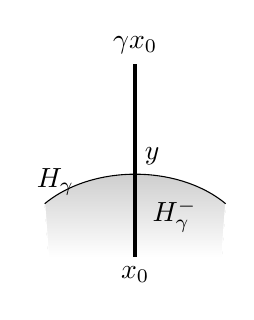
\begin{tikzpicture}[yscale=0.7]
	\coordinate (X0) at (0, 0);
	\coordinate (Y) at (0, 1.5);
	\coordinate (X1) at (0, 3.5);
		
	\fill[draw=white, shading=axis, top color=gray!40, bottom color=white] (1.1, 0) -- (40:1.5) arc[start angle=40, end angle=140, radius=1.5] -- (-1.1, 0) -- (1.1, 0);
	\draw[ultra thick] (X0) -- (X1);
	\draw (40:1.5) arc[start angle=40, end angle=140, radius=1.5] node[near end, left=0.5] {$H_\gamma$};
	\node[below] at (X0) {$x_0$};
	\node[above right] at (Y) {$y$};
	\node[above] at (X1) {$\gamma x_0$};
	\node at (0.5, 0.75) {$H_\gamma^-$};
\end{tikzpicture}\end{center}
一旦接受这些性质, 则 $x_0$ 连同 $H_\gamma$ 唯一确定 $\gamma x_0$: 它是 $x_0$ 对 $H_\gamma$ 的镜像, 而且
\begin{equation}\label{eqn:bisector-d}
	d(x_0, \gamma x_0) = 2d(x_0, y) = 2d(x_0, H_\gamma).
\end{equation}
下面证明 $H_\gamma$ 确实是中垂线.
\begin{lemma}\label{prop:bisector}
	沿用以上符号, 则 $H_\gamma$ 是经过 $y$ 点, 并在 $y$ 点与 $[x_0, \gamma x_0]$ 正交的唯一测地线.
\end{lemma}
\begin{proof}
	照搬命题 \ref{prop:geodesics} 的论证, 可以用 $\SL(2, \R)$ 的元素将 $x_0$ 和 $\gamma x_0$ 都搬到虚数轴上, 故无妨设
	\[ x_0 = is, \; \gamma x_0 = it, \quad 0 < s < t. \]
	代入命题 \ref{prop:hyperbolic-distance} 的距离公式, 得到
	\[ \tau \in H_\gamma \iff \frac{|\tau - is|^2}{s} = \frac{|\tau - it|^2}{t} \iff |\tau - is| = \sqrt{\frac{s}{t}} \cdot |\tau - it|. \]
	平面几何学的 Apollonius 圆定理或暴力计算说明这些 $\tau$ 的轨迹是圆 $\left\{ \tau: |\tau| = \sqrt{st} \right\}$ 和 $\mathcal{H}$ 之交. 代入命题 \ref{prop:geodesics} 知此为与 $[x,y]$ 正交的测地线.
\end{proof}

\begin{definition} \index{Dirichlet 区域 (Dirichlet domain)} \index[sym1]{$D(x_0)$}
	设 $x_0$ 非 $\overline{\Gamma}$ 的椭圆点. 以 $x_0 \in \mathcal{H}$ 为中心的 \emph{Dirichlet 区域}定义为 $\mathcal{H}$ 的闭子集
	\[ D(x_0) := \bigcap_{\gamma \in \overline{\Gamma} \smallsetminus \{1\}} H_\gamma^- = \left\{ x \in \mathcal{H}: \forall \gamma \in \overline{\Gamma},\; d(x, x_0) \leq d(x, \gamma x_0) \right\}. \] 
\end{definition}
基于对称性, 对任意 $\gamma \in \overline{\Gamma}$ 皆有 $\gamma D(x_0) = D(\gamma x_0)$.

称 $\mathcal{H}$ 的子集 $D$ 是\emph{测地凸}的, 如果对任意 $x,y \in D$, 测地线段 $[x,y]$ 全落在 $D$ 中. 显然测地凸子集都是道路连通的, 而任一族测地凸子集之交仍为测地凸.
\begin{proposition}
	对任意非椭圆点 $x_0 \in \mathcal{H}$ 和 $\gamma \in \overline{\Gamma} \smallsetminus \{1\}$, 子集 $H_\gamma^-$ 和 $D(x_0) \subset \mathcal{H}$ 皆为测地凸.
\end{proposition}
\begin{proof}
	仅须证明 $H_\gamma^-$ 情形. 设 $x, y \in H_\gamma^-$, 若 $[x,y]$ 在 $x_1$ 处穿出 $H_\gamma^-$, 则其后必在某点 $x_2$ 返回; 然而 $x_1, x_2 \in \partial H_\gamma^- = H_\gamma$ 而引理 \ref{prop:bisector} 说明 $H_\gamma$ 是测地线, 故必有 $[x_1, x_2] \subset H_\gamma$, 矛盾.
\end{proof}

\begin{proposition}\label{prop:Dirichlet-domain} \index{jibenquyu}
	若 $x_0$ 非椭圆点, 则 $D(x_0)$ 是 $\overline{\Gamma}$ 的连通基本区域, $\partial D(x_0)$ 为零测集.
\end{proposition}

引理 \ref{prop:elliptic-pt-discrete} 说明几乎所有 $x_0$ 皆非椭圆点.
\begin{proof}
	令 $x \in \mathcal{H}$. 因为 $\overline{\Gamma}$ 的作用正常, 在 \S\ref{sec:topological-group} 业已说明 $\overline{\Gamma} x_0$ 是 $\mathcal{H}$ 的离散子集, 故存在 $\gamma \in \overline{\Gamma}$ 使得 $d(x, \gamma x_0) = d(x, \overline{\Gamma} x_0)$. 按定义立见 $\gamma^{-1}x \in D(x_0)$. 于是 $\mathcal{H} = \bigcup_\gamma \gamma D(x_0)$.
	
	其次, $\overline{\Gamma} x_0$ 离散配上 \eqref{eqn:bisector-d} 导致对任意 $r > 0$, 测地球 $B_r := d(x_0, \cdot) < r$ 仅交有限多个 $H_\gamma$. 由于 $\mathcal{H} = \bigcup_{r > 0} B_r$, 这说明围出 $D(x_0)$ 的测地线族 $\left\{ H_\gamma : \gamma \in \overline{\Gamma} \right\}$ 是``局部有限''的. 由此循直观推得
	\begin{equation}\label{eqn:Dirichlet-interior}\begin{gathered}
		D(x_0)^\circ = \left\{ x \in \mathcal{H}: \forall \gamma \in \overline{\Gamma} \smallsetminus \{1\}, \; d(x, x_0) < d(x, \gamma x_0) \right\}, \\
		D(x_0) = \overline{D(x_0)^\circ}, \quad \mes(\partial D(x_0)) = 0.
	\end{gathered}\end{equation}
	同时 \eqref{eqn:Dirichlet-interior} 亦表明
	\[ \gamma = \gamma' \iff \gamma D(x_0)^\circ \cap \gamma' D(x_0)^\circ = D(\gamma x_0)^\circ \cap D(\gamma' x_0)^\circ \neq \emptyset; \]
	细节有请读者琢磨.
	
	最后来说明 $\left\{ \gamma D(x_0) : \gamma \in \overline{\Gamma} \right\}$ 局部有限. 设若不然, 存在紧集 $K$ 和一列相异的 $\delta_1, \delta_2, \ldots \in \overline{\Gamma}$, 使得对每个 $i \in \Z_{\geq 1}$ 都存在 $y_i \in K \cap \delta_i D(x_0)$; 命 $z_i := \delta_i^{-1} y_i$. 于是
	\begin{align*}
		d(x_0, \delta_i x_0) & \leq d(x_0, y_i) + d(y_i, \delta_i x_0) \\
		& = d(x_0, y_i) + d(z_i, x_0) \leq d(x_0, y_i) + d(y_i, x_0) \quad \left(\because \; z_i \in D(x_0)\right) \\
		& \leq 2 \sup_{y \in K} d(x_0, y) =: r,
	\end{align*}
	因为 $K$ 紧故 $r$ 有限. 无穷集 $\left\{ \delta_i x_0 \right\}_{i=1}^\infty$ 包含于紧集 $d(x_0, \cdot) \leq r$, 但这与 $\overline{\Gamma} x_0$ 离散矛盾.
\end{proof}

综上, $D(x_0)$ 是由一族测地线段围出的闭集. 具体确定 $D(x_0)$ 的样貌并非易事, 以下是最初步的例子.
\begin{example}\label{eg:Dirichlet-domain-full}
	取 $\overline{\Gamma} = \PSL(2,\Z)$ 和 $x_0 = it$, 其中 $t \in \R_{> 1}$. 今将说明 $D(x_0)$ 无非是 \eqref{eqn:fundamental-domain-full} 定义之 $\mathcal{F}$. 在 $H_\gamma^-$ 的定义中分别取 $\gamma$ 为 \eqref{eqn:S-T} 中的 $S, T, T^{-1}$, 用引理 \ref{prop:bisector} 直接计算
	\begin{equation*}
		H_S^- = \left\{ \tau : |\tau| \geq 1 \right\}, \quad H_T^- = \left\{ \tau : \Re(\tau) \leq \frac{1}{2} \right\}, \quad H_{T^{-1}}^- = \left\{ \tau : \Re(\tau) \geq -\frac{1}{2} \right\}.
	\end{equation*}
	因而 $D(x_0) \subset H_S^- \cap H_T^- \cap H_{T^{-1}}^- = \mathcal{F}$.

	一般来说, 对任意 $x_0$, 上半平面里对应于平移 $\gamma = \twomatrix{1}{t}{}{1}$ 的中垂线 $H_\gamma$ 必然是垂直线, 这点留给读者练手.
	
	假若 $D(x_0) \subsetneq \mathcal{F}$, 则因为 $D(x_0)$ 和 $\mathcal{F}$ 皆闭, $\mathcal{F} \smallsetminus D(x_0)$ 包含某个内点 $\tau \in \mathcal{F}^\circ$. 由于 $D(x_0)$ 是基本区域, 存在 $\gamma \in \overline{\Gamma} \smallsetminus \{1\}$ 使得 $\gamma\tau \in D(x_0) \subset \mathcal{F}$. 这与引理 \ref{prop:full-fundamental-domain-aux} 矛盾.
\end{example}

今后取定非椭圆点 $x_0$. 我们必须对 Dirichlet 区域 $D(x_0)$ 定义边的概念.
\begin{definition}[边, 顶点, 尖点]\label{def:sides} \index{jiandian} \index[sym1]{$D(x_0)^*$} \index{bian@边}
	我们规定:
	\begin{compactitem}
		\item $D(x_0)$ 的\emph{边}为形如 $\delta D(x_0) \cap D(x_0)$ 而长度非零的测地线段 (容许无穷长), 其中 $\delta \in \overline{\Gamma} \smallsetminus \{1\}$;
		\item 设 $\xi \in D(x_0)$, 若存在相异元 $\delta, \delta' \in \overline{\Gamma} \smallsetminus \{1\}$ 使得 $D(x_0) \cap \delta D(x_0) \cap \delta' D(x_0) = \{\xi\}$, 则称 $\xi$ 是 $D(x_0)$ 的\emph{顶点};
		\item 将 $\partial D(x_0)$ 中所有极大测地线段的无穷远点添入 $D(x_0)$ (或 $\partial D(x_0)$), 得到的集合记为 $D(x_0)^*$ (或 $\partial D(x_0)^*$). 若 $c \in D(x_0)^*$ 是两边的共同端点, 则称 $c$ 为 $D(x_0)^*$ 的\emph{尖点}; 我们也称尖点为 $D(x_0)$ 或 $D(x_0)^*$ 的无穷远顶点.
	\end{compactitem}
\end{definition}

在边的定义中, $\delta D(x_0) \cap D(x_0)$ 必然是 $\partial D(x_0)$ 的测地凸子集, 所以我们知道任一个边都包含于 $\partial D(x_0)$ 中的一个极大测地线段 (容许无穷长), 这种线段都是由某个 $H_\gamma$ 截出的. 显然, $\partial D(x_0)$ 中的极大测地线段无非是 $D(x_0)$ 直观意义上的边, 而定义 \ref{def:sides} 的边则与 $\left\{\delta D(x_0)\right\}_{\delta \in \overline{\Gamma}}$ 的铺砌方式有关. 稍加思索下图的``砌砖''现象, 就能明白 $\partial D(x_0)$ 的极大测地线段一般须加以细分, 才能给出 $D(x_0)$ 的边, 相应地也必须插入内角为 $\pi$ 的顶点.
\begin{center}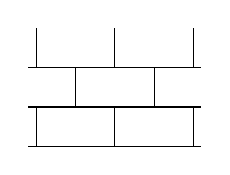
\begin{tikzpicture}[scale=0.5]
	\draw(-2.2, 1) -- (2.2, 1);
	\draw (-2.2, 0) -- (2.2, 0);
	\draw (-2.2, -1) -- (2.2, -1);
	\draw (-2,2) -- (-2,1); \draw (0,2) -- (0,1); \draw (2,2) -- (2,1);
	\draw (-1,1) -- (-1,0); \draw (1,1) -- (1,0);
	\draw (-2,0) -- (-2,-1); \draw (0,0)-- (0,-1); \draw (2,0) -- (2,-1);
\end{tikzpicture}\end{center}
需格外留意的是一条极大测地线段可能包含无穷多条边, 例子见 \cite[Example 10.1.1]{Bea95}; 鉴于基本区域的局部有限性, 此种情形仅可能对无穷长的极大测地线段发生.

直观上不难想见: $D(x_0)^*$ 的边和顶点至多可数, $\partial D(x_0)$ 是所有边之并, 两边至多交于一点 (必为顶点); 每个顶点正好是两边之交. 这些陈述都有严谨的论证, 可参看 \cite[\S 9.3]{Bea95}.

注意到 $D(x_0)^*$ 的无穷远点可以是开口之一端, 或者是尖点, 上半平面中图示如下:
\begin{center}\begin{tikzpicture}
	\fill[draw, shading=axis, bottom color=gray!40, top color=white] (-2, 2.5) -- (-2, 1) arc(90:0:1) -- (0,0) node[midway, below] {开口} arc(180:0:0.5) node[below] {尖点} arc(180:90:2) -- (3, 2.5) --cycle;
	\draw[white, ultra thick] (-2, 0) -- (-2, 2.5) -- (3, 2.5) -- (3, 0);
	\draw[dashed] (-2, 0) -- (3, 0) node[right] {$\R \sqcup \{\infty\}$};
	\node at (0, 2) {$D(x_0)$};
\end{tikzpicture}\end{center}
按定义 \ref{def:sides}, 任何尖点 $\xi$ 必为平行两边在无穷远处之交, 故 $\xi$ 处的内角为 $0$.

以下介绍边配对. 显见若 $S$ 为 $D(x_0)$ 的边, 那么使 $\delta D(x_0) \cap D(x_0) = S$ 的 $\delta \in \overline{\Gamma} \smallsetminus \{1\}$ 是唯一确定的, 又记为 $\delta_S$. 另一方面 $D(x_0) \cap \delta^{-1} D(x_0) = \delta^{-1} S$ 导致 $S' := \delta^{-1} S$ 也是 $D(x_0)$ 的边. 我们立刻看出
\[ (S')' = S, \quad \delta_{S'} = \delta_S^{-1}. \]

\begin{definition-proposition}[边配对]\label{prop:side-pairing} \index{bianpeidui@边配对 (side-pairing)}
	以上操作 $S \leftrightarrow S'$ 给出从 $D(x_0)$ 的边之间的配对; 使 $S' = \delta^{-1} S$ 之 $\delta \in \overline{\Gamma} \smallsetminus \{1\}$ 由 $S$ 唯一确定, 称为 $S$ 对应的配边元.
\end{definition-proposition}

考虑到未来对商空间的研究, 例如命题 \ref{prop:fundamental-domain-paste}, 我们在 $\partial D(x_0)^*$ 上引进如下等价关系: 记 $x \sim y$, 如果存在 $\delta \in \overline{\Gamma}$ 使得 $x = \delta y$ . 以下说明关系 $\sim$ 完全由边配对决定.
\begin{proposition}\label{prop:pairing-pasting}
	设相异元 $x, y \in \partial D(x_0)$ 满足 $x \sim y$, 那么存在配边元 $\delta_1, \ldots, \delta_n \in \overline{\Gamma}$ 使得 $x = \delta_1 \cdots \delta_n y$.
\end{proposition}
\begin{proof}
	取 $\delta \in \overline{\Gamma} \smallsetminus \{1\}$ 使得 $x = \delta y$, 那么 $x \in \delta D(x_0) \cap D(x_0)$. 设 $x$ 属于 $D(x_0)$ 的某边 $S$. 下图将边 $S$ 加粗显示, $x$ 标作 $\circ$, 描绘在 $x$ 附近典型的几何图像:
	\begin{center}\begin{tikzpicture}
		\coordinate (P1) at (-2, 0);
		\coordinate (P2) at (2, 0);
		\begin{scope}[shift = (P1)]
			\draw[ultra thick] (-1, 0) -- (1, 0) node[midway, above] {$\delta D(x_0)$} node[midway, below] {$D(x_0)$};
			\draw[fill=white] (0,0) circle[radius=1.8pt];
		\end{scope}
		\begin{scope}[shift = (P2)]
			\draw[ultra thick] (-1.5, 0) -- (0, 0);
			\draw (0, 0) -- (-1, 1);
			\draw (0, 0) -- (2, 0);
			\draw (0, 0) -- (1, 1);
			\draw (0, 0) -- (0, -1);
			\node at (1.7, 0.5) {$\delta D(x_0)$};
			\node at (-1.2, 0.4) {$\delta_1 D(x_0)$};
			\node at (-0.7, -0.7) {$D(x_0)$};
			\draw[dashed, -Latex] (-0.4, 0.8) arc(120:45:0.8);
			\draw[fill=white] (0, 0) circle[radius=1.8pt];
		\end{scope}
	\end{tikzpicture}\end{center}
	左图 $x$ 不是顶点, 这时 $\delta$ 是 $S$ 确定的配边元, $x = \delta y$ 给出所需表达式. 在右图情形下, 按箭头所示从 $D(x_0)$ 过渡到 $\delta_1 D(x_0), \ldots, \delta D(x_0)$, 每次都翻过一个含顶点 $x$ 之边, 并且对通过的边数 $n$ 作递归, 细述如下: $\delta_1$ 是 $S$ 确定的配边元. 如果 $\delta = \delta_1$ (即 $n=1$), 则和先前一样得出断言, 否则取
	\[ x'_0 := \delta_1 x_0, \quad y' := \delta_1 y \in \partial D(x'_0), \quad \delta' := \delta \delta_1^{-1} \in \overline{\Gamma} \smallsetminus \{1\}. \]
	于是 $x = \delta y = \delta' y'$, 而从 $\delta_1 D(x_0) = D(x'_0)$ 按上图过渡到 $\delta D(x_0) = \delta' D(x'_0)$, 通过 $n - 1$ 条边. 按递归假设, 存在 $D(x'_0)$ 的配边元 $\delta'_2, \ldots, \delta'_n$ 使得
	\[ x = \delta'_2 \cdots \delta'_n y' = \delta'_2 \cdots \delta'_n \delta_1 y. \]
	但是 $\delta'_i$ 是 $D(x'_0) = \delta_1 D(x_0)$ 的配边元蕴涵 $\delta_i := \delta_1^{-1} \delta'_i \delta_1$ 是 $D(x_0)$ 的配边元 ($i = 2, \ldots, n$). 因此
	\[ x = (\delta_1 \delta_2 \delta_1^{-1}) \cdots (\delta_1 \delta_n \delta_1^{-1}) \delta_1 y = \delta_1 \cdots \delta_n y, \]
	明所欲证.
\end{proof}


\begin{exercise}\label{exo:side-pairing-generation}
	证明所有配边元生成 $\overline{\Gamma}$.
	
	\begin{hint}
		类似命题 \ref{prop:pairing-pasting} 的论证, 从 $D(x_0)$ 一路穿墙到 $\delta D(x_0)$, 途经的边给出所需表达式.
	\end{hint}
\end{exercise}

\begin{remark}\label{rem:side-pairing}
	定义--命题 \ref{prop:side-pairing} 容许边和自身配对, 这就导致边还能够作如下细分, 以确保边配对 $S \leftrightarrow S'$ 无不动点. 以下设 $S' = S$, 记 $\gamma := \delta_S^{-1} \in \overline{\Gamma} \smallsetminus \{1\}$, 于是 $\gamma S = S$.
	\begin{compactenum}
		\item 假设 $S$ 有限长, 则 $\gamma$ 固定 $S$ 的中点 $\eta$. 例 \ref{eg:sliding} 表明 $\gamma|_S$ 必是对 $\eta$ 的反射. 将 $\eta$ 添入为顶点, 分 $S$ 为被 $\gamma$ 对调的两半.
		\item 若 $S' = S$ 无穷长, 则分两种情形考察 $\gamma$ 在 $S$ 上的作用.
		\begin{compactitem}
			\item 设 $S$ 两端无穷沿伸, 因此 $S$ 是一整条测地线. 例 \ref{eg:sliding} 表明 $\gamma$ 或者在 $S$ 上诱导平移, 这时它让 $D(x_0)$ 顺着 $S$ 滑动, 不可能给出边定义要求的 $D(x_0) \cap \gamma^{-1}D(x_0) = S$; 或者 $\gamma$ 是对某点 $\eta$ 的镜射, 这时仍向 $S$ 添入顶点 $\eta$, 分 $S$ 为被 $\gamma$ 对调的两半.
			\item 设 $S$ 仅有一端无穷延伸, 等距地等同于射线 $\R_{\geq 0}$. 那么 $\gamma$ 映包含 $S$ 的测地线为其自身, 并且保持 $S$ 两端不动. 依然应用例 \ref{eg:sliding} 来导出 $\gamma = 1$, 此无可能.
		\end{compactitem}
	\end{compactenum}

	以上两步新添的顶点 $\eta$ 都是椭圆点. 反之 $\partial D(x_0)$ 上的任何椭圆点 $\eta$ 也都是细分意义下的顶点: 设 $\eta$ 落在边 $S$ 上, 对任何 $\gamma \in \overline{\Gamma}_\eta \smallsetminus \{1\}$ (有限阶),
	\begin{compactitem}
		\item 或有 $\gamma S \neq S$, 直观可见 $\eta$ 已是顶点;
		\item 或有 $\gamma S = S$, 之前已论证 $\gamma|_S$ 此时将是镜射, 并且 $S$ 可被前述手续对半分割, 但镜射中点显然就是 $\eta$, 故 $\eta$ 是新添顶点.
	\end{compactitem}
	由于每条边至多细分为二, 若 $D(x_0)$ 边数有限, 细分后亦然; 这时边配对 $S \leftrightarrow S'$ 无不动点蕴涵细分后的边数为偶数.
\end{remark}

\begin{exercise}
	对例 \ref{eg:Dirichlet-domain-full} 的 Dirichlet 区域描述边的配对, 并按注记 \ref{rem:side-pairing} 予以细分.
\end{exercise}

记任意 $\xi \in \partial D(x_0)$ 处的内角为 $\theta(\xi)$, 容许 $\theta(\xi) = \pi$. 以下是双曲几何的一个基础结果, 也是尔后研究模曲线的必要工具.

\begin{proposition}\label{prop:angle-sum} \index[sym1]{eeta@$e(\eta)$}
	设 $\eta \in \partial D(x_0)$. 命 $e(\eta) := \left|\overline{\Gamma}_\eta\right|$, 如是则 $e(\eta) \in \Z_{\geq 1}$; 相对于命题 \ref{prop:pairing-pasting} 前的等价关系 $\sim$, 集合 $\left\{ \xi \in \partial D(x_0) : \xi \sim \eta\right\}$ 有限, 而且
	\[ \sum_{\substack{\xi \in \partial D(x_0) \\ \xi \sim \eta }} \theta(\xi) = \frac{2\pi}{e(\eta)}. \]
\end{proposition}
\begin{proof}
	命题 \ref{prop:stabilizer-finite-cyclic} 说明 $\overline{\Gamma}_\eta$ 有限. 我们有双射
	\begin{equation}\label{eqn:delta-xi}\begin{tikzcd}[row sep=small]
		\overline{\Gamma}_\eta \big\backslash \left\{ \delta \in \overline{\Gamma} : \eta \in \delta D(x_0) \right\} \arrow[r, "1:1"] & \left\{ \xi \in \partial D(x_0) : \xi \sim \eta \right\} \\
		\overline{\Gamma}_\eta \delta \arrow[mapsto, r] & \xi := \delta^{-1} \eta .
	\end{tikzcd}\end{equation}
	由于基本区域的局部有限性, $\left\{ \delta \in \overline{\Gamma} : \eta \in \delta D(x_0) \right\}$ 是有限集, 示意如下.
	\begin{center}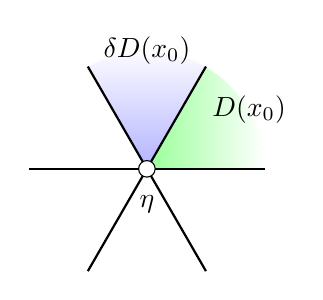
\begin{tikzpicture}[scale=1.5]
		\fill[draw=white, shading=axis, left color=green!40, right color=white] (0,0) -- (0:1) arc[start angle=0, end angle=60, radius=1] --cycle;
		\fill[draw=white, shading=axis, bottom color=blue!30, top color=white] (0,0) -- (60:1) arc[start angle=60, end angle=120, radius=1] --cycle;
		\foreach \a in {0, ..., 5}{
			\draw[thick] (0,0) -- (\a*60 : 1);
		}
		\node at (0, -0.3) {$\eta$};
		\node at (30:1) {$D(x_0)$};
		\filldraw[fill=white] (0,0) circle[radius=0.07];
		\node at (90:1) {$\delta D(x_0)$};
	\end{tikzpicture}\end{center}
	由此得出 $\left\{\xi \in \partial D(x_0): \xi \sim \eta \right\}$ 有限.
	
	记 $\delta D(x_0)$ 在 $\eta$ 处的内角为 $\Theta_\eta(\delta D(x_0))$, 因为 $\overline{\Gamma}$ 作用保角, 若 $\xi = \delta^{-1} \eta$ 则 $\theta(\xi) = \Theta_\xi(D(x_0)) = \Theta_\eta(\delta D(x_0))$. 鉴于 \eqref{eqn:delta-xi}, 在 $\eta$ 处的内角和遂写作
	\[ 2\pi = \sum_{\delta D(x_0) \ni \eta} \Theta_\eta(\delta D(x_0)) = \sum_{\xi \sim \eta} e(\eta) \theta(\xi). \]
	明所欲证.
\end{proof}

根据命题 \ref{prop:pairing-pasting}, 按边配对折叠 $D(x_0)$ 给出对 $\overline{\Gamma}$ 作用的商空间. 记 $y$ 为 $\eta \in \partial D(x_0)$ 在商空间中的像, 命题 \ref{prop:angle-sum} 的左式可以理解为 $y$ 周遭的角度和, 对折进 $y$ 的所有点 $\xi$ 作加总; 当 $e(\eta) > 1$ 时结果小于 $2\pi$. 这就表明将椭圆点附近的双曲度量降到商空间上会遇到一些麻烦; 就度量几何的观点, 也可以设想商空间在 $y$ 处有个锥奇点. 关于椭圆点造成的种种困难, 我们以后还会碰上.
